\documentclass[main.tex]{subfiles}
\pagenumbering{arabic}
\begin{document}

\setdoublesep{0.35700 em}  % 'Bond Spacing'
\setatomsep{1.78500 em}    % 'Fixed Length'
\setbondoffset{0.18265 em} % 'Margin Width'
\newcommand{\bondwidth}{0.06642 em} % 'Line Width'
\setbondstyle{line width = \bondwidth}


\chapter[Organic Chemistry ]{Organic Chemistry}

\begin{marginfigure}
      \includegraphics{chapter15/figure1}
   \end{marginfigure}
\lettrine[lines=4]{\color{black!45}T}{he} previous chapter have covered the chemical properties of what we call inorganic compounds. These are for example cooking salt (\ce{NaCl}), water (\ce{H2O}) or ammonia (\ce{NH3}). This chapter covers organic compounds, which are chemicals based on carbon and hydrogen. We used organic compounds in the form of numerous materials such as fuels, perfumes, plastics or drugs. They all have common properties, from their smells to their powerful action. We will address first the naming of organic compounds as well as the properties of these important chemicals. Finally we will address the different groups of functional atoms that give unique properties to molecules such as caffeine or cocaine.
\definesubmol{CH2}{CH_2}



\begin{marginfigure}%LEARNING GOALS BOX
\begin{mytcbox}{GOALS}

\begin{enumerate}[label=\protect\circled{\color{white}\arabic*}]
\item Identify organic chemicals
\item Name linear hydrocarbons
\item Name cyclic hydrocarbons
\item Name hydrocarbons with substituents
\item Identify functional groups
\end{enumerate}
\end{mytcbox}
\end{marginfigure}%LEARNING GOALS BOX

\begin{marginfigure}[0.5cm]
\begin{tcolorbox}[enhanced,colback=red!5!white,colframe=black!50!red,boxrule=1pt,
  arc=0pt,outer arc=0pt,drop heavy lifted shadow]
\faGears\ 
\docenvdef{Discussion:} Think about any drug you have taken recently. Paste its structure and indicate at least one functional group in the molecule. \end{tcolorbox}
 \end{marginfigure}

\begin{marginfigure}[2cm]%%%%%%%% MARGIN FIGURE
\includegraphics{chapter15/figure2}
\caption{Methane (\ce{CH4}) is used as a fuel for ovens, homes, water heaters. }
\end{marginfigure}%%%%%%% MARGIN FIGURE


\section{\color{blue!30!black}{Alkanes}}
This first section will introduce organic chemistry, covering the most simple organic compounds: the alkanes. Alkanes simply contain carbon and hydrogen and are also called hydrocarbons. First you will be introduced to a few organic chemicals without paying to much attention to their names. Then, you will learn about a series of different organic formulas that can represent the same compound. Finally, you will learn the naming rule of alkanes, which basically extend to other--more complex--organic chemicals.
\sloppy
?\begin{description}
\item[\docfilehook{\smallpencil Identifying organic compounds}{Identifying organic compounds}] How do we know when we have an organic or an inorganic chemical? Organic chemicals are based on carbon and hydrogen. They can contain other nonmetallic elements such as oxygen, nitrogen or sulfur. Here a few examples: \ce{CH4}, \ce{C2H6}, \ce{C6H6} or \ce{CH3COOH}. Mind that carbonates (\ce{Na2CO3}), carbon monoxide (\ce{CO}) or carbon dioxide (\ce{CO2}) are not organic compounds. 

\item[\docfilehook{\smallpencil Methane}{Methane}] The simplest organic compound is methane: \ce{CH4}. Methane is a fuel and the main constituent of natural gas. Going back a few chapters, the Lewis structure of methane is:
\begin{center}\chemfig{C(-[2]H)(-[4]H)(-[6]H)(-[8]H)}\hspace{0.5cm}\textcolor{blue}{Methane, \ce{CH4}}\end{center}
This structure is very representative in this chapter as it shows that each carbon atom has to be connected to four different atoms.

\item[\docfilehook{\smallpencil Alkanes}{Alkanes}] Alkanes are simple organic compounds made of Carbon and Hydrogen with all carbons connected by means of simple bonds--these are single lines to represent the connections between atoms. The naming of alkanes results of adding a prefix to the sufix \emph{ane}. The prefix depends on the number of carbons in the molecule. Table \ref{table12:2} shows a list of the different prefixes. For example, the alkane with one carbon is called methane. Another example of alkanes would be ethane that contains two carbons:
\begin{center}\chemfig{C(-[2]H)(-[4]H)(-[6]H)-C(-[2]H)(-[6]H)-H} \hspace{0.5cm}\textcolor{blue}{Ethane, \ce{C2H6}}\end{center}
or propane:
\begin{center}\chemfig{C(-[2]H)(-[4]H)(-[6]H)-C(-[2]H)(-[6]H)-C(-[2]H)(-[6]H)-H} \hspace{0.5cm}\textcolor{blue}{Propane, \ce{C3H8}}\end{center}




\begin{marginfigure}[-5cm]%%%%%%%MARGIN FIGURE
 \label{table12:2}
\begin{tcolorbox}[tab2,tabularx={X|Y}]%%%% FANCY COLOR TABLE
\# Carbons & prefix              \\\hline\hline
1 &    Meth           \\\hline
2 &    Eth           \\\hline
3 &   Pro          \\\hline
4 &    But           \\\hline
5 &    Pent           \\\hline
6 &    Hex           \\\hline
7 &    Hepta           \\\hline
8 &    Octa           \\\hline
9 &    Nona           \\\hline
10 &    Deca                  
\end{tcolorbox}%%%% FANCY COLOR TABLE
\caption{Prefixed for alkane naming.}
 \end{marginfigure}%%%%%%%MARGIN FIGURE

\item[\docfilehook{\smallpencil General formula for alkanes}{General formula for alkanes}] At this point we saw two different alkanes: methane (\ce{CH4}), butane (\ce{C2H6}) and propane (\ce{C3H8}). The general formula for an alkane with $n$ carbon atoms is:

\begin{equation}
 \text{C}_n\text{H}_{2n+2}
 \label{formula12.1}
 \end{equation}
 \resizeableyellownote{2.5}{1}{Add  Formula \textcolor{blue}{\ref{formula12.1}} to your flashcard.}
 As an example, the formula for methane ($n=1$) is $ CH_{4}$ and the formula for octane ($n=8$) is $ C_8H_{18}$.
\begin{marginfigure}%%%%%%%% MARGIN FIGURE
\includegraphics{chapter15/figure3}
\caption{Hydrocarbons are made of carbon and hydrogen. }
\end{marginfigure}%%%%%%% MARGIN FIGURE
\begin{example} %%%%%%%%%%%%%%%%%%%%%%%% EXAMPLE BOX
Write down the molecular formula for decane and pentane.
\\
\textlcsc{ \textcolor{dgreen}{\Large \textbf{Solution}} }\\
Using Equation \ref{formula12.1} we have that the molecular formula for decane ($n=10$) would be: \ce{C10H22}. Similarly, the molecular formula for pentane ($n=5$) would be: \ce{C5H12}.
\\
\faDiamond\ \textlcsc{ \textcolor{dgreen}{\Large \textbf{Study Check}} }\\
Name the alkane with formula \ce{C7H16} and give the formula for nonane.
\\
\flushright{  \small Answer: heptane, \ce{C9H20}.}
\end{example}%%%%%%%%%%%%%%%%%%%%%%%% EXAMPLE BOX
\begin{marginfigure}[2cm]%%%%%%%% MARGIN FIGURE
\includegraphics{chapter15/figure4}
\caption{The octane rating of gas is a standard measure of the performance of engine fuels, originally determined by mixing a gasoline made entirely of heptane and 2,2,4-trimethylpentane (a highly branched octane).}
\end{marginfigure}%%%%%%% MARGIN FIGURE
\newpage
\item[\docfilehook{\smallpencil Alkanes contain \ce{CH3} and \ce{CH2} units}{Alkanes contain \ce{CH3} and \ce{CH2} units}] Let us analyze the formula of propane. In this formula there are two different types of carbons. One is the end of the chain carbon, in the left and in the right. The other type of carbon is the central carbon. The extremes are bounded to three hydrogen, whereas the central is bounded to two hydrogens.
\begin{center}\chemfig{C(-[2]@{B}H)(-[4]@{A}H)(-[6]H)-C(-[2]H@{E})(-[6]H)-C(-[2]H@{C})(-[6]H)-H@{D}} \end{center}
\chemmove{
  \draw[
    fill=purple,
    draw=purple,
    fill opacity=.2,
    rounded corners=2pt
  ]
    ([xshift=-5pt,yshift=-25pt]A.south west) rectangle ([xshift=5pt,yshift=5pt]B.north east) ;
        \draw[
    fill=purple,
    draw=purple,
    fill opacity=.2,
    rounded corners=2pt
  ]
        ([xshift=-10pt,yshift=-43pt]C.south west) rectangle ([xshift=5pt,yshift=30pt]D.north east) ;
         \draw[
    fill=red,
    draw=red,
    fill opacity=.2,
    rounded corners=2pt
  ]
        ([xshift=-10pt,yshift=-40pt]E.south west) rectangle ([xshift=5pt,yshift=10pt]E.north east) ;
}
The extremes are indeed \ce{CH3} units and the center is a \ce{CH2} unit. So, another way to represent ethane would be:
\begin{center}\chemfig{CH_3-!{CH2}-CH_3} \hspace{0.5cm}\textcolor{blue}{Ethane, \ce{C2H6}}\end{center}
At this point you have seen three different ways to represent organic molecules. Let us use propane as an example. One is the  \emph{molecular formula}, which in the case of propane is \ce{C3H8}. Another different way to represent propane is with its \emph{expanded structural formula}, that is by representing all C and all H in the molecule. Another molecular representation is the \emph{condensed structural formula}, that is by using \ce{CH3} and \ce{CH2} units. Here the three formulas:
\begin{center}\begin{tikzpicture}[help lines/.style={thin,draw=black!50}]
\node at (0,0) {\chemfig{C_3H_8}};
\node at (0,-2) {\textcolor{blue}{\begin{tabular}{c} molecular \\ formula \end{tabular}}};
\node at (4,0) {\chemfig{CH_3-CH_2-CH_3}};
\node at (4,-2) {\textcolor{blue}{\begin{tabular}{c} condensed \\ formula \end{tabular}}};
\node at (8,0) {\chemfig{C(-[2]H)(-[4]H)(-[6]H)-C(-[2]H)(-[6]H)-C(-[2]H)(-[6]H)-H}};
\node at (8,-2) {\textcolor{blue}{\begin{tabular}{c} expanded structural \\ formula \end{tabular}}};
\end{tikzpicture}\end{center}












\begin{figure*}[h] % FUL FIGURE

\centering
\fontfamily{ppl}\selectfont
\begin{tabular}{lll}
\toprule
\rowcolor{black!45}
Number of Carbons & Prefix & Condensed Structural formula \\
\midrule
1 & Meth & \chemfig{CH_4}  \\
2 & Eth & \chemfig{CH_3-CH_3}  \\
3 & Prop & \chemfig{CH_3-CH_2-CH_3}  \\
4 & But & \chemfig{CH_3-CH_2-CH_2-CH_3}  \\
5 & Pent & \chemfig{CH_3-CH_2-CH_2-CH_2-CH_3}  \\
6 & Hex & \chemfig{CH_3-CH_2-CH_2-CH_2-CH_2-CH_3}  \\
7 & Hepta & \chemfig{CH_3-CH_2-CH_2-CH_2-CH_2-CH_2-CH_3}  \\
8 & Oct & \chemfig{CH_3-CH_2-CH_2-CH_2-CH_2-CH_2-CH_2-CH_3}  \\
9 & Non & \chemfig{CH_3-CH_2-CH_2-CH_2-CH_2-CH_2-CH_2-CH_2-CH_3}  \\
\bottomrule\end{tabular}
%\caption{The name of alkanes is related to the number of carbons in its formula.}
\label{table12:1}

\end{figure*} % FUL FIGURE


\begin{example} %%%%%%%%%%%%%%%%%%%%%%%% EXAMPLE BOX
Write down the condensed and expanded formulas for pentane.
\\
\textlcsc{ \textcolor{dgreen}{\Large \textbf{Solution}} }\\
Pentane has five carbons, hence its condensed formula will have two \ce{CH3} units and three \ce{CH2} units:
\begin{center}\chemfig{CH_3-CH_2-CH_2-CH_2-CH_3}\end{center}
The expanded formula for pentane would be:
\begin{center}\chemfig{C(-[2]H)(-[4]H)(-[6]H)-C(-[2]H)(-[6]H)-C(-[2]H)(-[6]H)-C(-[2]H)(-[6]H)-C(-[2]H)(-[6]H)-H} \end{center}
\faDiamond\ \textlcsc{ \textcolor{dgreen}{\Large \textbf{Study Check}} }\\
Write down the condensed and expanded formulas for heptane.
\\
 \begin{flushright} \small Answer: \small 
 \setpolymerdelim()\chemfig{H-C(-[2]H)(-[6]H) -[@{A,0.5}:0,2]C(-[2]H)(-[6]H) -[@{B,0.5}:0,2]C(-[2]H)(-[6]H)-H }\makebraces(15pt,15pt){$\scriptstyle\!\!5$}{A}{B}; 
  \setpolymerdelim()\chemfig{CH_3 -[@{A,0.5}:0,2]CH_2 -[@{B,0.5}:0,2]CH_3 }\makebraces(5pt,5pt){$\scriptstyle\!\!5$}{A}{B}

 \end{flushright}

\end{example}%%%%%%%%%%%%%%%%%%%%%%%% EXAMPLE BOX






\item[\docfilehook{\smallpencil ZigZag}{ZigZag}] Let us analyze the structure of propane again. This molecule has three carbons in the form of a C-C chain such as: C-C-C. However, C-C chains with more than more three carbons are not linear. So instead of representing propane as:
\begin{center}\chemfig{H_3C-!{CH2}-CH_3} \end{center}
we could represent this molecule by means of a zigzag:

\begin{center}\chemfig{H_3C-[:45]!{CH2}-[:-45]CH_3} \hspace{0.5cm}\textcolor{blue}{Propane, \ce{C3H8}}\end{center}
Another example would be butane:
\begin{center}\chemfig{H_3C-[:45]!{CH2}-[:-45]CH_2-[:45]CH_3} \hspace{0.5cm}\textcolor{blue}{Butane, \ce{C4H10}}\end{center}

\item[\docfilehook{\smallpencil Skeletal formula}{Skeletal formula}] A final way to represent molecules in this chapter is simply using lines. This is called the skeletal formula, as you only represent the C-C skeleton of the molecule. Let us use hexane an an example. We can represent this molecule as in this two ways:
\begin{center}\begin{tikzpicture}[help lines/.style={thin,draw=black!50}]
\node at (0,0) {\chemfig{H_3C-[:45]!{CH2}-[:-45]CH_2-[:45]CH_2-[:-45]CH_2-[:45]CH_3} };
\node at (0,-2) {\textcolor{blue}{condensed formula}};
\node at (6,0) {\chemfig{-[:45]-[:-45]-[:45]-[:-45]-[:45]}};
\node at (6,-2) {\textcolor{blue}{skeletal formula}};
\end{tikzpicture}\end{center}
The ending of a skeletal formula represents a \ce{CH3} and the points in between represents \ce{CH2}. 

\begin{example} %%%%%%%%%%%%%%%%%%%%%%%% EXAMPLE BOX
Write down the condensed and skeletal formulas for heptane.
\\
\textlcsc{ \textcolor{dgreen}{\Large \textbf{Solution}} }\\
Heptane has seven carbons, hence its condensed formula will have two \ce{CH3} units and five \ce{CH2} units:
\begin{center}\chemfig{H_3C-[:45]!{CH2}-[:-45]CH_2-[:45]CH_2-[:-45]CH_2-[:45]CH_2-[:-45]CH_3}\end{center}
The skeletal formula for would be:
\begin{center}\chemfig{-[:45]-[:-45]-[:45]-[:-45]-[:45]-[:-45]} \end{center}
\faDiamond\ \textlcsc{ \textcolor{dgreen}{\Large \textbf{Study Check}} }\\
Draw the skeletal formula of decane.
\\
\flushright{  \small Answer: \chemfig{-[:45]-[:-45]-[:45]-[:-45]-[:45]-[:-45]-[:45]-[:-45]-[:45]}}
\end{example}%%%%%%%%%%%%%%%%%%%%%%%% EXAMPLE BOX


\end{description}

\section{\color{blue!30!black}{Cycloalkanes}}
This section deals with cyclic alkanes. Alkanes are perfect examples of hydrocarbons, with C-C chains and all carbon atoms saturates with hydrogen. Cycloalkanes are in essence alkanes that have a cyclic structure. We will cover the molecular, condensed and skeletal formulas for these chemicals.
\sloppy
\begin{marginfigure}%%%%%%%% MARGIN FIGURE
\includegraphics{chapter15/figure5}
\caption{Cyclononane contains 9 carbons in a cycle. \\ \textcolor{red}{\textbf{Q:} What is the molecular formula Cyclononane?} }
\end{marginfigure}%%%%%%% MARGIN FIGURE
\begin{description}
\item[\docfilehook{\smallpencil Cyclic alkanes}{Cyclic alkanes}] Let us use the expanded estructure of hexane as an example. 
\begin{center}\chemfig{C(-[:90]H)(-[:180]H)(-[:-90]H)-C(-[:90]H)(-[:-90]H)-C(-[:90]H)(-[:-90]H)-C(-[:90]H)(-[:-90]H)-C(-[:90]H)(-[:-90]H)-C(-[:90]H)(-[:-90]H)-H   }\end{center}
A cycloalkane results of eliminating the left and right hydrogen and connecting the molecule in the form of a cycle:
\begin{center}\chemfig{H-C(-[:90]H)(-[:-90]@A)-CH_2-CH_2-CH_2-CH_2-C(-[:90]H)(-[:-90]@B)-H   }\end{center}
\chemmove{\draw[shorten >=4pt]
(A).. controls +(-90:1cm) and +(-90:1cm).. (B);}

As the most stable structure for six lines is the hexagon. The results looks like

\begin{center}\chemfig{H_2C*6(-CH_2-CH_2-CH_2-CH_2-H_2C-[,,2])}\hspace{1cm} or \hspace{1cm}\chemfig{*6(------)}  \hspace{0.5cm}\textcolor{blue}{cyclohexane}\end{center}

\item[\docfilehook{\smallpencil Naming cyloalkanes}{Naming cyloalkanes}] The naming of alkanes and cycloalkanes is very similar. You just need to add the cyclo prefix to the name. For example, the alkane with five carbons is called pentane. The corresponding cycloalkane is called cyclopentane:
\begin{center}\chemfig{CH_2*5(-CH_2-CH_2-CH_2-CH_2-[,,2])}\hspace{1cm} or \hspace{1cm}\chemfig{*5(------)}  \hspace{0.5cm}\textcolor{blue}{Cyclopentane}\end{center}

\begin{marginfigure}[-10cm]%%%%%%%% MARGIN FIGURE
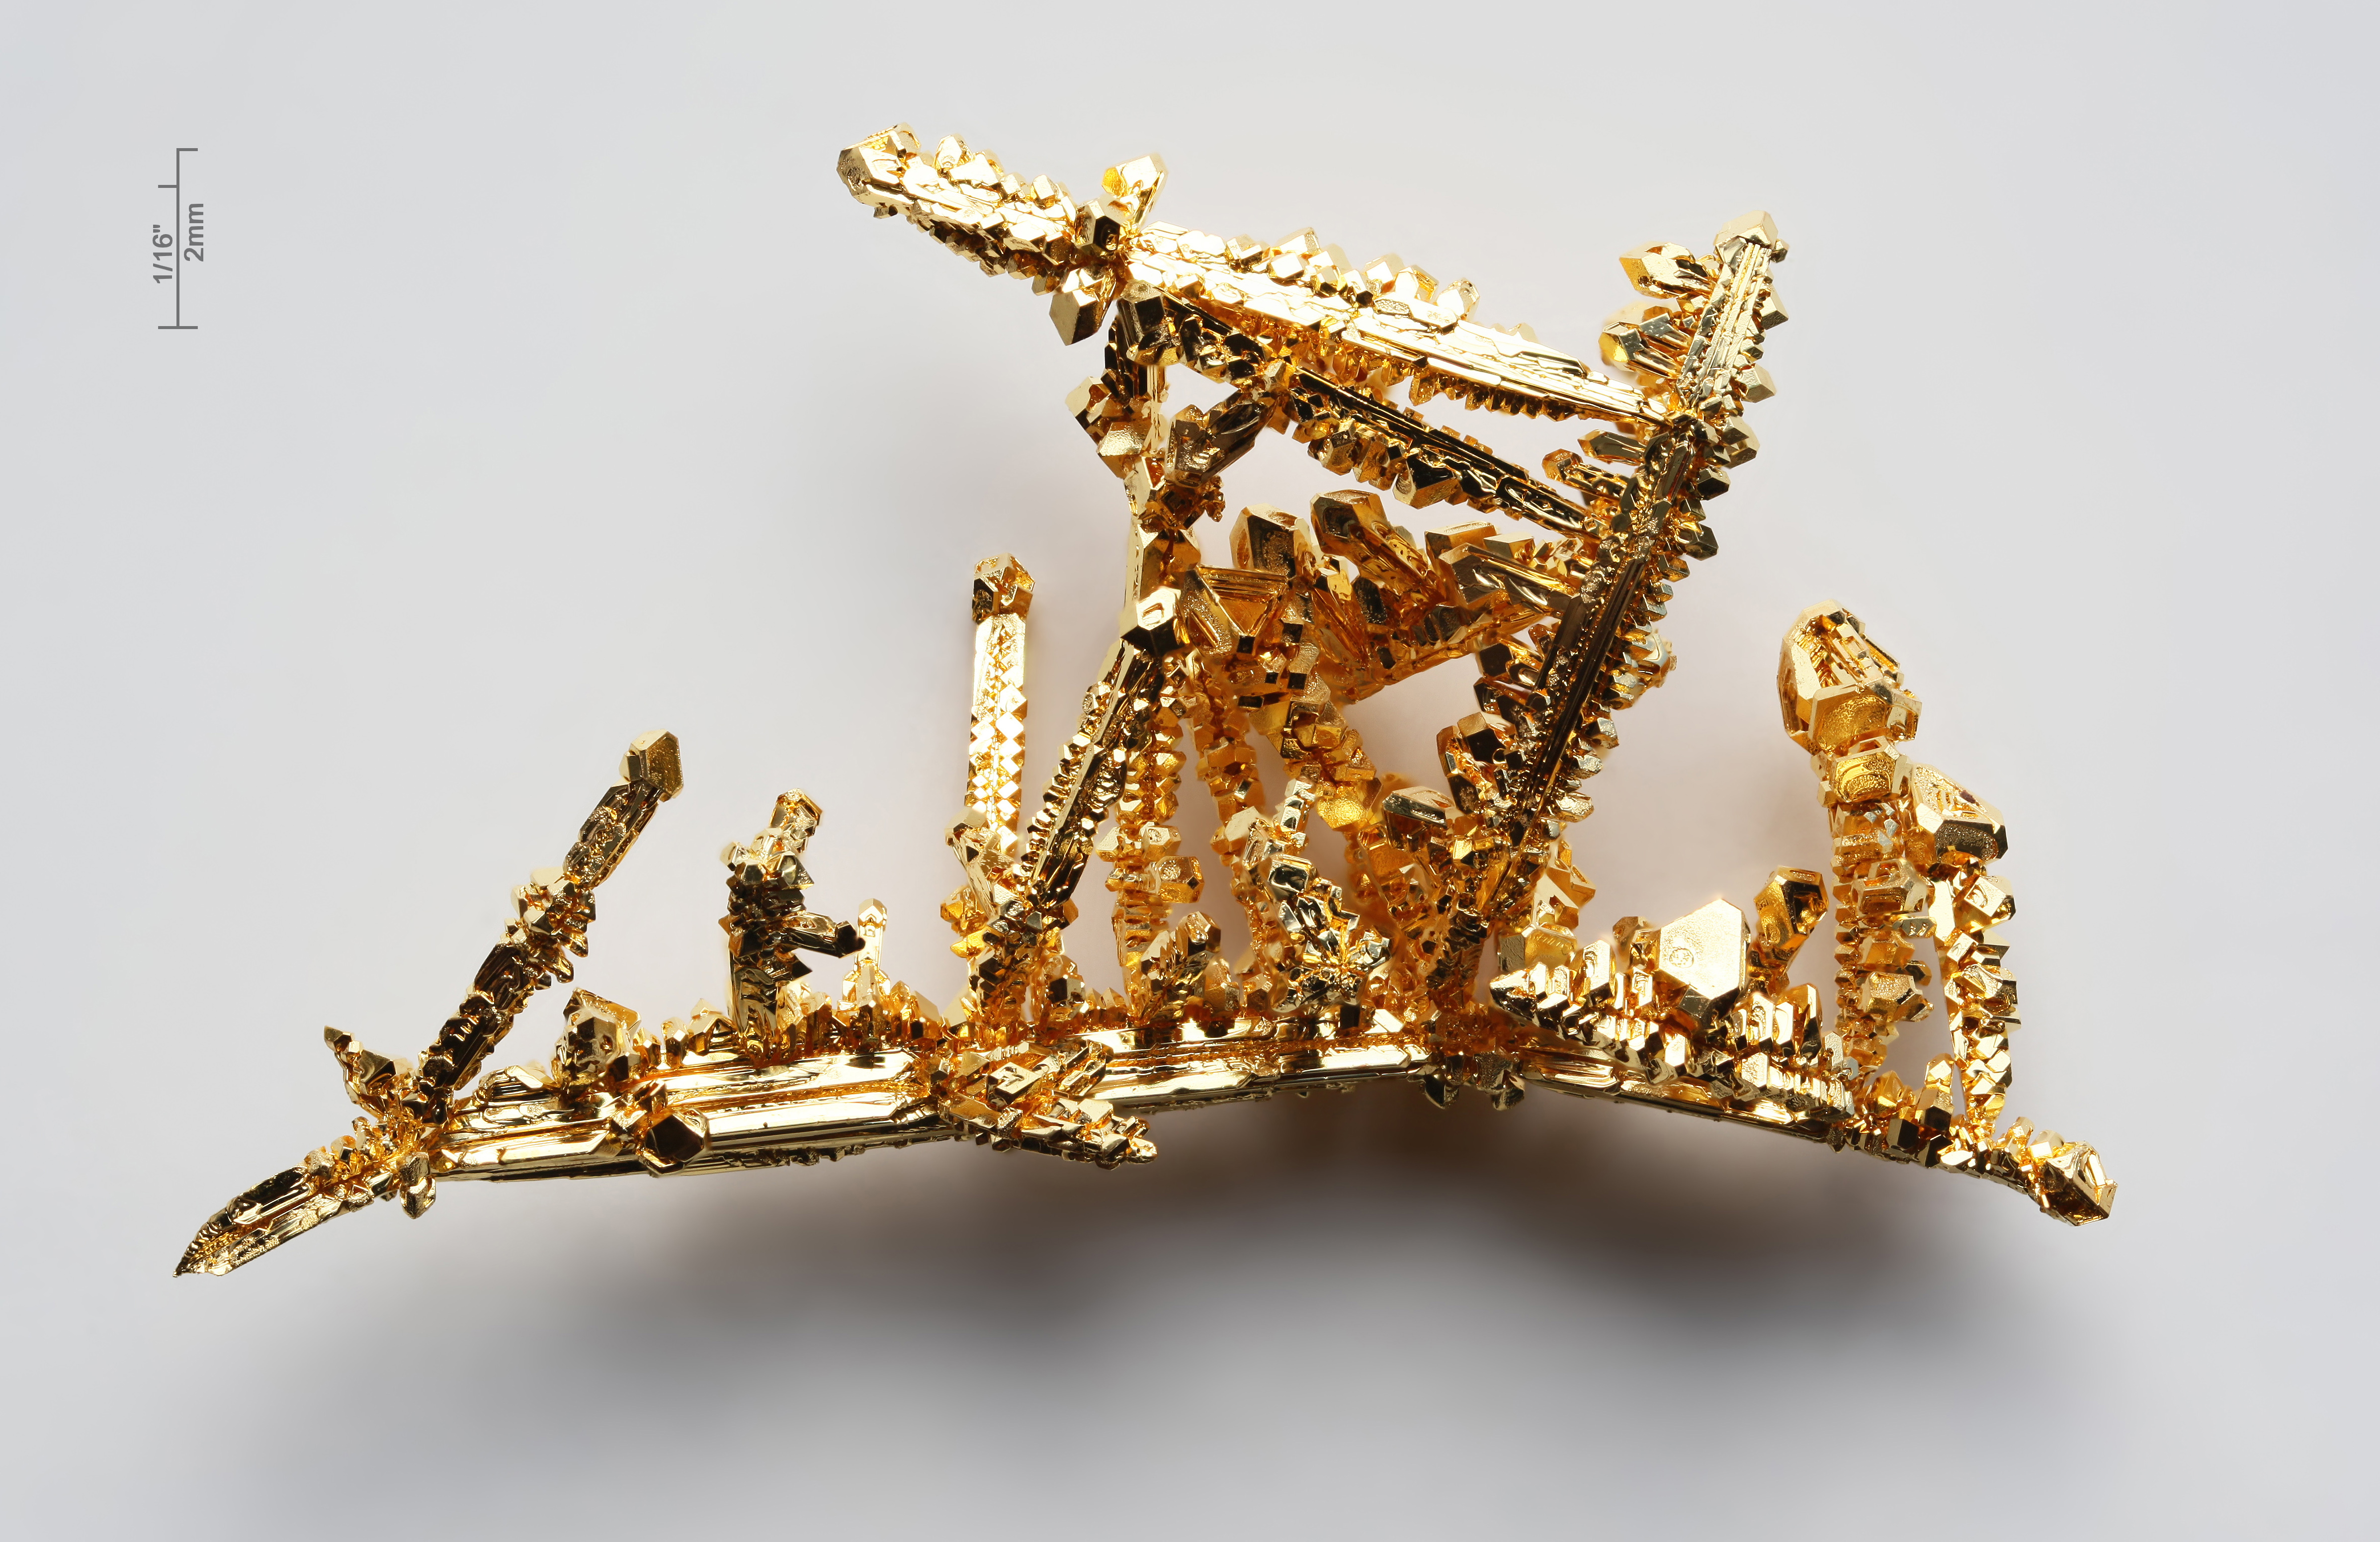
\includegraphics{chapter15/figure6}
\caption{Cyclohexane has a chair shape. \\ \textcolor{red}{\textbf{Q:} How many H are there in cyclohexane?} }
\end{marginfigure}%%%%%%% MARGIN FIGURE
\begin{marginfigure}[-1cm]%%%%%%%% MARGIN FIGURE
\includegraphics[width=0.7\columnwidth]{chapter15/figure7}
\caption{Cyclopropane has only three carbons and a lot tension in its cycle. \\ \textcolor{red}{\textbf{Q:} Would cyclopropane be a stable of unstable molecule?} }
\end{marginfigure}%%%%%%% MARGIN FIGURE
\begin{example} %%%%%%%%%%%%%%%%%%%%%%%% EXAMPLE BOX
Write down the condensed structure and name the following cycloalkane:
\begin{center}\chemfig{*4(----)} \end{center}
\textlcsc{ \textcolor{dgreen}{\Large \textbf{Solution}} }\\
The cycloalkane has four carbons and its name is cylcobutane. Its condensed structure is 
\begin{center}\chemfig{CH_2*4(-CH_2-CH_2-CH_2-[,,2])}\end{center}
\faDiamond\ \textlcsc{ \textcolor{dgreen}{\Large \textbf{Study Check}} }\\
Write down the condensed structure and name the following cycloalkane:
\begin{center}\chemfig{*3(---)} \end{center}
\flushright{  \small Answer: cyclopropane, \chemfig{CH_2*3(-CH_2-CH_2-[,,2])} }
\end{example}%%%%%%%%%%%%%%%%%%%%%%%% EXAMPLE BOX


\item[\docfilehook{\smallpencil General formula for cycloalkanes}{General formula for cycloalkanes}]  The general formula for an cycloalkane with $n$ carbon atoms is:

\begin{equation}
 \text{C}_n\text{H}_{2n}
 \label{formula12.2}
 \end{equation}
 \resizeableyellownote{2.5}{1}{Add  Formula \textcolor{blue}{\ref{formula12.2}} to your flashcard.}
 As an example, the formula for cyclopropane ($n=4$) is \ce{C4H_{8}} and the formula for cycloctane ($n=8$) is \ce{C_8H_{16}}.

\begin{example} %%%%%%%%%%%%%%%%%%%%%%%% EXAMPLE BOX
Write down the molecular formula for cyclodecane and cyclopentane.
\\
\textlcsc{ \textcolor{dgreen}{\Large \textbf{Solution}} }\\
Using Equation \ref{formula12.2} we have that the molecular formula for cyclodecane ($n=10$) would be: \ce{C10H20}. Similarly, the molecular formula for cyclopentane ($n=5$) would be: \ce{C5H10}.
\\
\faDiamond\ \textlcsc{ \textcolor{dgreen}{\Large \textbf{Study Check}} }\\
Name the alkane with formula \ce{C7H14} and give the formula for cyclononane.
\\
\flushright{  \small Answer: cycloheptane, \ce{C9H18}.}
\end{example}%%%%%%%%%%%%%%%%%%%%%%%% EXAMPLE BOX
\end{description}

\begin{marginfigure}[0cm]%%%%%%%MARGIN FIGURE
 \label{table12:2}
\begin{tcolorbox}[tab2,tabularx={XX|Y}]%%%% FANCY COLOR TABLE
Substituents && name              \\\hline\hline
\chemfig{CH_3-[:0,1]} &&    Methyl          \\\hline
\chemfig{CH_3CH_2-[:0,1]} &&    Ethyl           \\\hline
\chemfig{CH_3CH_2CH_2-[:0,1]} &&   Propyl          \\\hline
\vspace{0.2cm} \chemfig{H_3C-[:0,1]CH(-[:90,1]\phantom{L})(-[:0,1]CH_3)}
 &&    Isopropyl           \\\hline
 \vspace{0.2cm} \chemfig{H_3C-[:0,1]C(-[:-90,1]CH_3)(-[:90,1]\phantom{L})(-[:0,1]CH_3)}
 &&   t-butyl           \\\hline
\chemfig{F-[:0,1]} &&    Fluoro     \\\hline      
 \chemfig{Cl-[:0,1]}&&    Chloro   \\\hline        
 \chemfig{Br-[:0,1]} &&    Bromo   \\\hline        
 \chemfig{I-[:0,1]} &&    Iodo          \\\hline  
 \chemfig{NH_2-[:0,1]} &&    Amino     \\\hline   
 \chemfig{NO_2-[:0,1]} &&   Nitro    \\\hline   
 \chemfig{CH_2=CH-[:0,1]} &&   Vinyl    

            
\end{tcolorbox}%%%% FANCY COLOR TABLE
\caption{Name of some substituents.}
 \end{marginfigure}%%%%%%%MARGIN FIGURE



\section{\color{blue!30!black}{Alkanes with substituyents}}
At this point you should be familiar with alkanes. These organic compounds are carbon-based chemicals made of lines of C-C hydrocarbon chains. Often times these hydrocarbons have other groups of atoms attached to the hydrocarbon chains and these are called substituents. This section cover the naming of alkanes with substituents. Here an example of an alkane and an alkane with a substituent:
\begin{center}\chemname{\chemfig{CH_3-CH_2-CH_3}}{Propane}\hspace{1cm}
\chemname{\chemfig{CH_2(-[:90,1]NO_2)-CH_2-CH_3}}{Nitropropane}\end{center}
\sloppy
\begin{description}

\item[\docfilehook{\smallpencil Substituents}{Substituents}] There are many different substituents which can be found connected to an alkane chain. Their names are indicated in Figure 1.8. The easiest substituents are halogens and atoms of chorine (\chemfig{Cl-[:0,1]}), bromine (\chemfig{Br-[:0,1]}) or iodine (\chemfig{I-[:0,1]}) can connect to an alkane. The name of these substituents is chloro, bromo and iodo. Other substituents can contain carbon, like a methyl (\chemfig{CH_3-[:0,1]}) or a ethyl (\chemfig{CH_3CH_2-[:0,1]}). There are even more complex substituents such as tert-butyl




\item[\docfilehook{\smallpencil Alkanes with a single substituent}{Alkanes with a single substituent}] Let us consider the following example. The condensed formula for propane is
\begin{center} \chemfig{CH_3-CH_2-CH_3} \hspace{0.5cm}\textcolor{blue}{Propane}\end{center}
Now, this would be propane with a substituent:
\begin{center} \chemfig{CH_2(-[:90,1]Br)-CH_2-CH_3} \hspace{0.5cm}\textcolor{blue}{Bromopropane}\end{center}
As you can see a bromine atom substitutes one of the hydrogen atoms of the second first of the molecule (starting from the left).

\item[\docfilehook{\smallpencil Alkanes with two or more equal substituents}{Alkanes with two or more equal substituents}] In the same way as when you have a single bromine atom attached to propane, you can also have two \chemfig{Br-[:0,1]}. In this case you need to use the prefix \emph{di} to indicate there are two identical bromines. For example, the name of the following molecule would be
\begin{center} \chemfig{CH(-[:90,1]Br)(-[:-90,1]Br)-CH_2-CH_3} \hspace{0.5cm}\textcolor{blue}{Dibromopropane}\end{center}
Similarly, you should use the prefix \emph{tri} for three equal substituents.

\begin{example} %%%%%%%%%%%%%%%%%%%%%%%% EXAMPLE BOX
Name the following hydrocarbon:
\begin{center} \chemfig{CH_3-CH_2-CH_2-CH(-[:90,1]I)(-[:-90,1]I)}\end{center}
\textlcsc{ \textcolor{dgreen}{\Large \textbf{Solution}} }\\
The carbon chain has four carbons and hence the ending of the name would be: butane. Also there are two iodines (iodo substituents) attached to the carbon chain. As there are two of the same iodo atoms, we need to use the prefix \emph{di}. The full name would be: Dioiodobutane.
\\
\faDiamond\ \textlcsc{ \textcolor{dgreen}{\Large \textbf{Study Check}} }\\
Name the following hydrocarbon:
\begin{center} \chemfig{CH_3-CH_2-CH_2-CH_2-C(-[:0,1]F)(-[:90,1]F)(-[:-90,1]F)}\end{center}
\flushright{  \small Answer: Trifluoropentane. }
\end{example}%%%%%%%%%%%%%%%%%%%%%%%% EXAMPLE BOX



\item[\docfilehook{\smallpencil Alkanes with different substituents}{Alkanes with different substituents}] 
Now imagine you have two different halogens as substituents: \chemfig{Br-[:0,1]} and \chemfig{I-[:0,1]} like in next example

\begin{center} \chemfig{CH(-[:90,1]Br)(-[:-90,1]I)-CH_2-CH_3}\end{center}
As they have different names you cannot use the prefix \emph{di}. Still, when you indicate the names of the substituents you need to order them according to the \emph{abc}. So bromo goes first in the name and iodo after. You also need to separate the different substituents with a '-'. The final name of the hydrocarbon above would be: Bromo-Iodopropane.



\begin{example} %%%%%%%%%%%%%%%%%%%%%%%% EXAMPLE BOX
Name the following hydrocarbon:
\begin{center} \chemfig{CH_3-C(-[:90,1]F)(-[:-90,1]I)-Br}\end{center}
\textlcsc{ \textcolor{dgreen}{\Large \textbf{Solution}} }\\
The carbon chain has two carbons and hence the ending of the name would be: ethane. Also there are three different substituents: iodine (iodo substituents), bromine (bromo substituents) and fluorine (fluoro substituents). We need to order them according to the \emph{abc}, hence the order would be: bromo, then fluoro and finally iodo. The full name of the alkane would be: Bromo-Fluoro-Iodoethane.
\\
\faDiamond\ \textlcsc{ \textcolor{dgreen}{\Large \textbf{Study Check}} }\\
Name the following hydrocarbon:
\begin{center} \chemfig{CH_3CH_2CH_2-C(-[:90,1]F)(-[:-90,1]F)-Br}\end{center}
\flushright{  \small Answer: Bromodifluorobutane. }
\end{example}%%%%%%%%%%%%%%%%%%%%%%%% EXAMPLE BOX


\item[\docfilehook{\smallpencil Numbering the chain}{Numbering the chain}] Substituents are atoms or groups of atoms that can plug into a alkane chain. You could envision plugging these atoms at different points of the chain. For example:
\begin{center} \chemfig{CH_3-CH(-[:90,1]Br)-CH_3} \hspace{0.5cm}or\hspace{0.5cm} \chemfig{CH_2(-[:90,1]Br)-CH_2-CH_3}\end{center}

In the right example Br is plugged to the left C atom, whereas in left example C is plugged to the middle carbon. Hence, it is important first, to learn how to number a hydrocarbon chain. Let us use propane as an example. This molecule has three atoms. In order to number the chain, you start by selecting the extreme that is the closest to the substituent, and use this carbon as number one. Next carbon would be carbon number two and so on until you arrive to carbon number three. 
\begin{center}\chemfig{C\chembelow[1ex]{}{\tiny \textcolor{red}{1}}H(-[:90]Br)-C\chembelow[1ex]{}{\tiny \textcolor{red}{2}}H_2-C\chembelow[1ex]{}{\tiny \textcolor{red}{3}}H_3}\end{center}
As the Br atom in the carbon number one, the name of the molecule would be: 1-bromopropane or simply bromopropane. Differently, when the substituent is in a carbon different than one, you need to indicate that location. For example:

\begin{center} \chemfig{CH_3-CH(-[:90,1]Br)-CH_3} \hspace{0.5cm}\textcolor{blue}{2-Bromopropane}\end{center}




\begin{example} %%%%%%%%%%%%%%%%%%%%%%%% EXAMPLE BOX
Name the following hydrocarbon:
\begin{center} \chemfig{CH_3-CH(-[:90,1]CH_3)(-CH(-[:-90,1]I)-Br)}\end{center}
\textlcsc{ \textcolor{dgreen}{\Large \textbf{Solution}} }\\
First we find the ending of the name: as the molecule has three carbons in the main chain, the ending of the name would be: propane. Then we need to number the chain so that the number one carbon is the closest to the substituents:
\begin{center} \chemfig{C\chembelow[1ex]{}{\tiny \textcolor{red}{3}}H_3-C\chembelow[1ex]{}{\tiny \textcolor{red}{2}}H(-[:90,1]CH_3)(-C\chemabove[2ex]{}{\tiny \textcolor{red}{1}}H(-[:-90,1]I)-Br)}\end{center}
A methyl is connected to carbon two, and two halogens, a iodo and a bromo are connected to carbon number one. The substituents are: 2-methyl, 1-bromo, 1-iodo. If we order them: 1-bromo-1-iodo-2-methyl. And the final name would be: 1-bromo-1-iodo-2-methylpropane.
\\
\faDiamond\ \textlcsc{ \textcolor{dgreen}{\Large \textbf{Study Check}} }\\
Name the following hydrocarbon:
\begin{center} \chemfig{CH_3-C(-[:90,1]CH_3)(-[:-90,1]F)(-CH_2-I)}\end{center}\flushright{  \small Answer: 1-iodo-2-fluoro-2-methylpropane. }
\end{example}%%%%%%%%%%%%%%%%%%%%%%%% EXAMPLE BOX




\item[\docfilehook{\smallpencil Finding the longest chain}{Finding the longest the chain}] Alkanes with substituents are more complex than simple alkanes and often time they contain more than one hydrocarbon chain. Therefore, one can envision several ways to number the chain. The rule is to locate the longest chain. Let us use the following hydrocarbon. How many chains can you find, and which is the longest chain?

\begin{center} \chemfig{CH_3-CH_2-CH(-[:90]CH_2-CH_2-CH_2-CH_3)-CH_3} \end{center}
The answer should be three chains. Let me highlight the three different possibilities and the number of atoms in each chain:



\begin{center}
 \chemfig{@{A}CH_3-CH_2-CH(-[:90]CH_2-CH_2-CH_2-CH_3)-CH_3@{B}}\chemmove{
   \fill [fill=red, fill opacity=.1,line width=.00pt] ([xshift=0pt,yshift=-10pt]A.south west) rectangle ([xshift=0pt,yshift=10pt]B.north east) ;
}\hspace{0.5cm}\textcolor{blue}{4 Carbons} \end{center}\vspace{0.5cm}
\begin{center} \chemfig{@{A}CH_3-CH_2-C@{B}H(-[:90]C@{C}H_2-CH_2-CH_2-CH_3@{D})-CH_3}\chemmove{
   \fill [fill=red, fill opacity=.1,line width=.00pt] ([xshift=0pt,yshift=-10pt]A.south west) rectangle ([xshift=3.5pt,yshift=8pt]B.north east) ;
      \fill [fill=red, fill opacity=.1,line width=.00pt] ([xshift=-8pt,yshift=8pt]B.north west) rectangle ([xshift=-1pt,yshift=6pt]C.north east) ;
            \fill [fill=red, fill opacity=.1,line width=.00pt] ([xshift=11pt,yshift=-8pt]C.south west) rectangle ([xshift=0pt,yshift=13.0pt]D.north east) ;
}\hspace{0.5cm}\textcolor{blue}{7 Carbons} \end{center}\vspace{0.5cm}
\begin{center} \chemfig{CH_3-CH_2-C@{B}H(-[:90]C@{C}H_2-CH_2-CH_2-CH_3@{D})-CH_3@{E}} \chemmove{
      \fill [fill=red, fill opacity=.1,line width=.00pt] ([xshift=-10pt,yshift=2.6pt]B.north west) rectangle ([xshift=-1pt,yshift=6pt]C.north east) ;
            \fill [fill=red, fill opacity=.1,line width=.00pt] ([xshift=11pt,yshift=-8pt]C.south west) rectangle ([xshift=0pt,yshift=13.0pt]D.north east) ;
               \fill [fill=red, fill opacity=.1,line width=.00pt] ([xshift=-10pt,yshift=-10pt]B.south west) rectangle ([xshift=3.5pt,yshift=9.5pt]E.north east) ;
}\hspace{0.5cm}\textcolor{blue}{6 Carbons} \end{center}
As the longest chain has seven carbons, the name of the molecule would be heptane. Still you need to add the substituents before that name. After you locate the longest chain you need to number the chain so that the substituents are located the closest to the carbon number one the possible:


\begin{center}\vspace{1cm}\chemfig{@{A}C\chembelow[1ex]{}{\tiny \textcolor{red}{1}}H_3-C\chembelow[1ex]{}{\tiny \textcolor{red}{2}}H_2-C\chembelow[1ex]{}{\tiny \textcolor{red}{3}}@{B}H(-[:90]C\chemabove[2ex]{}{\tiny \textcolor{red}{4}}@{C}H_2-C\chemabove[2ex]{}{\tiny \textcolor{red}{5}}H_2-C\chemabove[2ex]{}{\tiny \textcolor{red}{6}}H_2-C\chemabove[2ex]{}{\tiny \textcolor{red}{7}}H_3@{D})-CH_3}\chemmove{
   \fill [fill=red, fill opacity=.1,line width=.00pt] ([xshift=0pt,yshift=-12pt]A.south west) rectangle ([xshift=3.5pt,yshift=8pt]B.north east) ;
      \fill [fill=red, fill opacity=.1,line width=.00pt] ([xshift=-8pt,yshift=8pt]B.north west) rectangle ([xshift=-1pt,yshift=8pt]C.north east) ;
            \fill [fill=red, fill opacity=.1,line width=.00pt] ([xshift=11pt,yshift=-8pt]C.south west) rectangle ([xshift=0pt,yshift=15.0pt]D.north east) ;
}\end{center}

So in carbon number three a methyl is located. Hence the final name of the molecule would be: 3-methylheptane.



\begin{example} %%%%%%%%%%%%%%%%%%%%%%%% EXAMPLE BOX
Name the following hydrocarbon:
\begin{center} \chemfig{CH_3-CH_2-C(-[:90]CH_3)(-[:-90]CH_2-CH_2-CH_3)-CH_3} \end{center}
\textlcsc{ \textcolor{dgreen}{\Large \textbf{Solution}} }\\
First we locate the longest chain. We have five possible chains, and the longest one has six carbons. Hence the name of the hydrocarbon would be hexane. Now we need to number the carbons so that we start numbering the closes to the substituents the possible.
\begin{center} \chemfig{C\chembelow[1ex]{}{\tiny \textcolor{red}{1}}H_3-C\chembelow[1ex]{}{\tiny \textcolor{red}{2}}H_2-C\chembelow[1ex]{}{\tiny \textcolor{red}{3}}(-[:90]CH_3)(-[:-90]C\chembelow[1ex]{}{\tiny \textcolor{red}{4}}H_2-C\chembelow[1ex]{}{\tiny \textcolor{red}{5}}H_2-C\chembelow[1ex]{}{\tiny \textcolor{red}{6}}H_3)-CH_3} \end{center}\vspace{0.5cm}
We have two methyl connected to carbon number three. Hence the final name will be: 3-dimethylhexane.
\\
\faDiamond\ \textlcsc{ \textcolor{dgreen}{\Large \textbf{Study Check}} }\\
Name the following hydrocarbon:
\begin{center} \chemfig{CH_3-CH_2-C(-[:90]CH_2-CH_2-CH_2-CH_3)(-[:-90]CH_2-CH_2-CH_3)-CH_3} \end{center}
\flushright{  \small Answer: 4-ethyl-4-methyloctane. }
\end{example}%%%%%%%%%%%%%%%%%%%%%%%% EXAMPLE BOX



\end{description}




\section{\color{blue!30!black}{Cylcoalkanes with substituyents}}
Cycloalkanes are cyclic alkanes. This section covers the naming of cycloalkanes with substituents. The naming rules are the same as the rules for naming alkanes. This means first you will find the ending on the name by counting the number of carbons. Then you will locate each substituent and number the carbon chain so that these substituents are close to carbon number one. All substituents have a number depending on the carbon number. Finally, all substituents should be order according to the \emph{abc}.
\sloppy
\begin{description}
\item[\docfilehook{\smallpencil Cylcoalkanes with one substituyent}{Cylcoalkanes with one substituyent}] Let us take a look at the following cycloalkane:
\definesubmol\Me[H_3C]{CH_3}
\begin{center}\chemfig{*6(----(-!\Me)---)} \end{center}
this is a cyclohexane connected to a methyl substituent. As there is only one substituents, there is no need to number the carbon chain. Hence the name would be: methylcyclohexane.

\item[\docfilehook{\smallpencil Cylcoalkanes with two substituyent}{Cylcoalkanes with one substituyent}] Let us take a look at the following cycloalkane:
\begin{center}\chemfig{*6(---(-F)-(-!\Me)---)} \end{center}
this is a cyclopentane connected to two different substituents: a methyl and a fluoro. In order to name this molecule we need to number the carbons first, and there are two different ways to number the cyclohexane ring:
\definesubmol\A{(-[,-0.3,,,draw=none]\textcolor{red}{1})}
\definesubmol\B{(-[,-0.3,,,draw=none]\textcolor{red}{2})}
\definesubmol\C{(-[,-0.3,,,draw=none]\textcolor{red}{3})}
\definesubmol\D{(-[,-0.3,,,draw=none]\textcolor{red}{4})}
\definesubmol\E{(-[,-0.3,,,draw=none]\textcolor{red}{5})}
\definesubmol\F{(-[,-0.3,,,draw=none]\textcolor{red}{6})}
\newcommand\X[1]{(-[,-0.3,,,draw=none]{#1})}

\begin{center}
\chemname{\chemfig{*6((!\D)-(!\E)-(!\F)-(!\A)(-F)-(!\B)(-!\Me)-(!\C)--)} }{1-Fluoro-2-methylcyclohexane}
\hspace{4.5cm}
\chemname{\chemfig{*6((!\E)-(!\D)-(!\C)-(!\B)(-F)-(!\A)(-!\Me)-(!\F)--)} }{(wrong) Fluoro-1-methylcyclohexane}
\end{center}
we will choose the name that gives the lowest numbers: 1-Fluoro-2-methylcyclohexane.




\item[\docfilehook{\smallpencil Cylcoalkanes with repeated substituyent}{Cylcoalkanes with repeated substituyent}] Let us take a look at the following cycloalkane, which has two repeated fluorine substituents:
\begin{center}\chemfig{*6(---(-F)-(-F)---)} \end{center}
After numbering the chain:
\begin{center}\chemname{\chemfig{*6((!\E)-(!\D)-(!\C)-(!\B)(-F)-(!\A)(-F)-(!\F)--)} }{}\end{center}
The name would be: 1,2-difluorocyclohexane.
\begin{example} %%%%%%%%%%%%%%%%%%%%%%%% EXAMPLE BOX
Name the following hydrocarbon:
\begin{center}\chemname{\chemfig{*5(--(-F)--(-Br)-)} }{}\end{center}
\textlcsc{ \textcolor{dgreen}{\Large \textbf{Solution}} }\\
The molecule is a cyclopentane with two substituents: fluoro and bromo. I will start numbering in bromo and continue until bromo. This way I will have small numbers and follow the abc rule:
\begin{center}\chemname{\chemfig{*5(--(!\C)(-F)-(!\B)-(!\A)(-Br)-)} }{}\end{center}
And the name of the molecule would be: 1-bromo-3-fluorocyclopentane.\\
\faDiamond\ \textlcsc{ \textcolor{dgreen}{\Large \textbf{Study Check}} }\\
Name the following hydrocarbon:
\begin{center}\chemname{\chemfig{*4(-(-F)-(-I)-(-Br)-)} }{}\end{center}
\flushright{  \small Answer: 1-bromo-3-fluoro-2-bromocyclopropane. }
\end{example}%%%%%%%%%%%%%%%%%%%%%%%% EXAMPLE BOX


\end{description}




\begin{marginfigure}[7cm]%%%%%%%MARGIN FIGURE
 \label{table12:3}
\begin{tcolorbox}[tab2,tabularx={XX|Y}]%%%% FANCY COLOR TABLE
Functional groups && name              \\\hline\hline
\chemfig{C(-[3]R_1)(-[-3]R_2)(=C(-[1]R_3)(-[-1]R_4))}&&    Alkene        \\\hline
   \chemfig{R-C~C-R'} &&    Alkyne       \\\hline
\chemfig{R-OH} &&    Alcohol         \\\hline
 \chemfig{R-SH}&&    Thiol          \\\hline
\chemfig{R-O-R'} &&   Ether         \\\hline
   \chemfig{R-C(=[:90]O)-R'}      &&   Ketone         \\\hline
    \chemfig{R-C(=[:90]O)-H}     &&   Aldehyde         \\\hline
     \chemfig{R-C(=[:90]O)-OH}    &&   Carboxylic acid         \\\hline
     \chemfig{R-C(=[:90]O)-O-R'}    &&   Ester         \\\hline
   \chemfig{R-N(-[:90]R')(-R'')}      &&   Amine         \\\hline
   \chemfig{R-C(=[:90]O)(-N(-R')((-[:90]R'')))}      &&   Amide        
\end{tcolorbox}%%%% FANCY COLOR TABLE
\caption{Name of functional groups.}
 \end{marginfigure}%%%%%%%MARGIN FIGURE
\section{\color{blue!30!black}{Molecular diversity}}
The previous sections covered hydrocarbons, either alkanes or cyclocalkanes. Both alkanes and cyclocalkanes are molecules based on carbon and hydrogen. This section will introduce the idea of functional group. You have certainly taken painkillers for a headache or over-the-counter drugs to get over a cold. Maybe you drink coffee and perhaps you like tea. All these medications as well as drinks contain active organic molecules. These active molecules differ from plain  hydrocarbons, which are simply made of carbon and hydrogen. Active molecules contain functional groups such as alcohol, ethers, carboxylic acids, amines, amides or aromatic groups. These groups of atoms have a specific function and give activity to the molecule. The goal of this section is not for you to identify the action mechanisms of these complex active molecules, but simply to identify the different groups.

\sloppy
\begin{description}
\item[\docfilehook{\smallpencil Alkene group: double bonds}{Alkene group: double bonds}] Alkenes contain at least one double bond between carbons. An example would be:
\begin{center}\chemfig{\chemfig{C(-[3]CH_3)(-[-3]H)(=C(-[1]H)(-[-1]CH_3))}}\hspace{1cm} or\hspace{1cm}\chemfig{CH_3CH_2-HC=CH-CH_3}\end{center}
As both sides of an alkene can be connected to different hydrocarbon chains we normally represent this as:
\begin{center}\chemfig{C(-[3]R_1)(-[-3]R_2)(=C(-[1]R_3)(-[-1]R_4))}\hspace{0.5cm}\textcolor{blue}{Alkene}\end{center}
where R and R' represents any hydrocarbon chain.


%\begin{marginfigure}[0cm]%%%%%%%% MARGIN FIGURE
%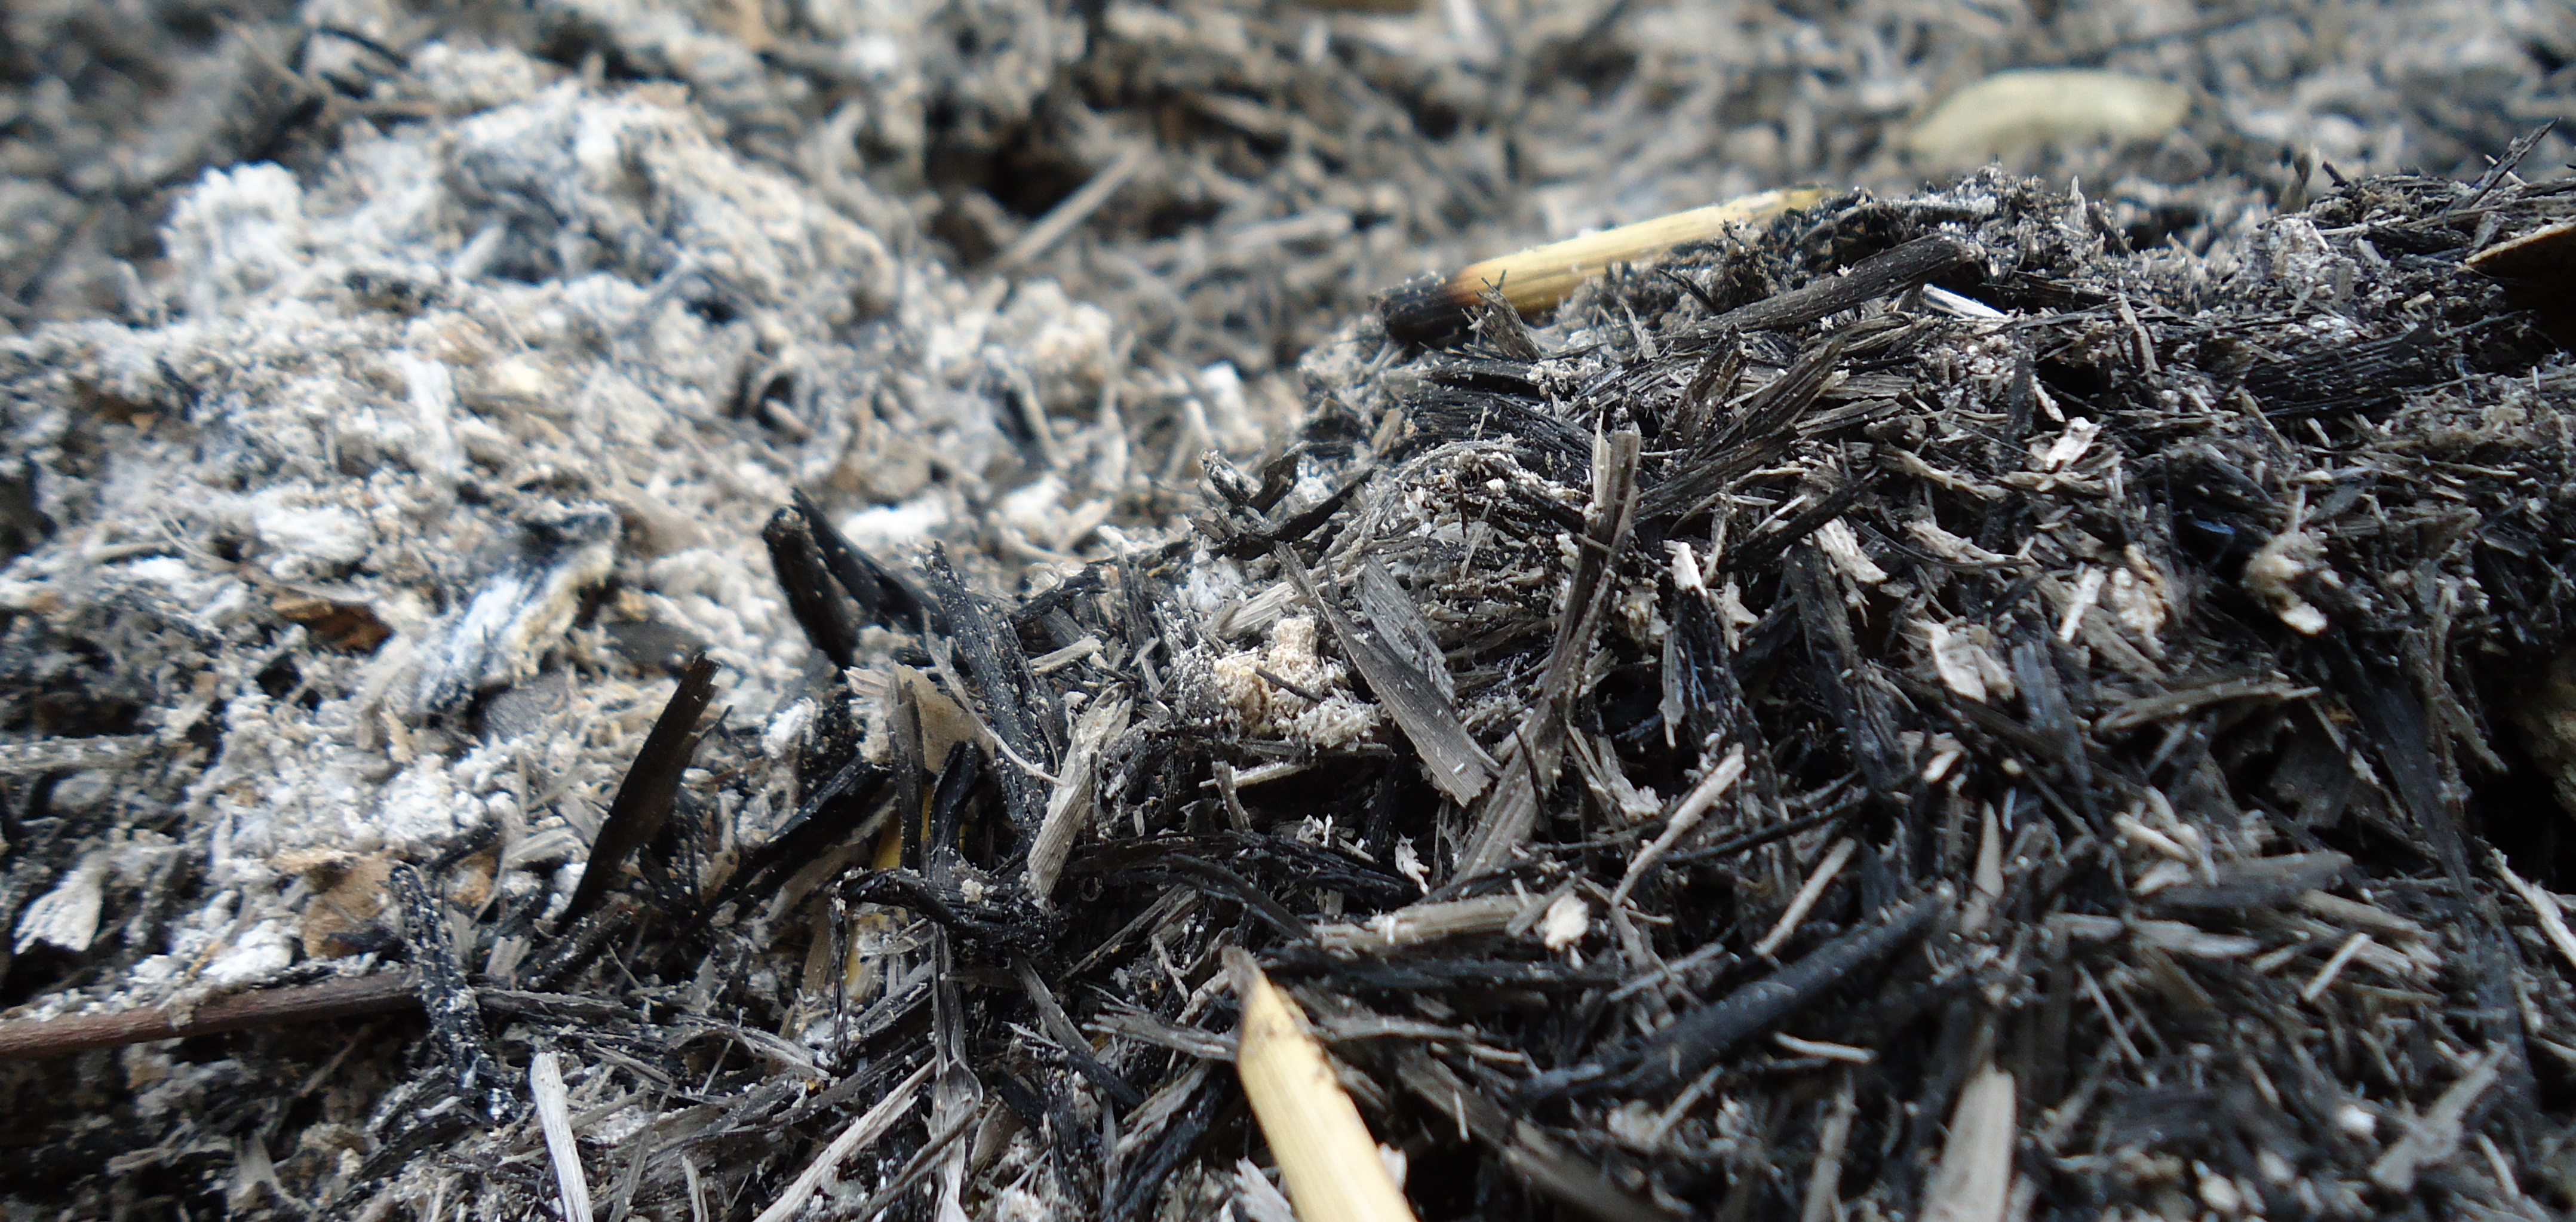
\includegraphics[width=0.4\columnwidth]{chapter15/figure8}
%\caption{Acetone, the smallest ketone with three carbons, is also known as nail polish remover.\\ \textcolor{red}{\textbf{Q:} What is the formula for acetone?} }
%\end{marginfigure}%%%%%%% MARGIN FIGURE

\item[\docfilehook{\smallpencil Alkyne group: tripe bonds}{Alkyne group: tripe bonds}] Alkenes contain at least one tripple bond between carbons. An example would be:
\begin{center}\chemfig{CH_3-C~C-C{(}CH_3{)}_3}\hspace{1cm} or\hspace{1cm}\chemfig{CH_3-CH(-[:90]CH_3)-C~C-CH_3}\end{center}
Again we could use R and R' to represent any hydrocarbon chain:
\begin{center}\chemfig{R-C~C-R'}\hspace{0.5cm}\textcolor{blue}{Alkyne}\end{center}

\begin{example} %%%%%%%%%%%%%%%%%%%%%%%% EXAMPLE BOX
Identify the alkene and alkyne groups in the molecule:
\begin{center}\chemfig{H_2C=C(-[1]CH_2-CH~CH)(-[-1]H)}\end{center}
\textlcsc{ \textcolor{dgreen}{\Large \textbf{Solution}} }\\
A double bond is carbon atoms sharing two pairs of electrons, whereas a triple bond is a pair of atoms sharing three pairs of electrons. They are represented with a double and triple line, respectively. In the question:
\begin{center}\chemfig{H_2\phantom{}@{A}C=\phantom{}@{B}C(-[1]CH_2-H\phantom{}@{C}C~\phantom{}@{D}CH)(-[-1]H)}\end{center}
\chemmove{
   \fill [fill=red, fill opacity=.1,line width=.00pt] ([xshift=0pt,yshift=-10pt]A.south west) rectangle ([xshift=0pt,yshift=10pt]B.north east) ;
      \fill [fill=red, fill opacity=.1,line width=.00pt] ([xshift=0pt,yshift=-10pt]C.south west) rectangle ([xshift=0pt,yshift=10pt]D.north east)  ;
}

\faDiamond\ \textlcsc{ \textcolor{dgreen}{\Large \textbf{Study Check}} }\\
Identify the alkene and alkyne groups in the molecule:
\begin{center}\chemfig{H_3C-C~C-C(-[-1]H)(-[1]C(-[3]H)(=C(-[-1]CH_3)(-[1]CH_2-C~C-CH_3)))}\end{center}
\end{example}%%%%%%%%%%%%%%%%%%%%%%%% EXAMPLE BOX

\begin{marginfigure}[-5cm]%%%%%%%% MARGIN FIGURE
\begin{center}
\chemfig{?=[::+72]*5(-N=(-=[::-72]*5(-[,,,2]HN-[,,2](=-[::-36]*5(=N-(=-[::-72]*5(-NH-[,,1]?=-=))
-=-))-=-))-=-)}\end{center}
\caption{Porphirin has several amine groups. \\ \textcolor{red}{\textbf{Q:} How many amine groups has porphirin?} }
\end{marginfigure}%%%%%%% MARGIN FIGURE
\begin{marginfigure}[0cm]%%%%%%%% MARGIN FIGURE
\begin{center}\chemfig{*6(-=-(-O-[::-60](-[::-60])=[::+60]O)=(-(=[::+60]O)-[::-60]OH)-=)}
\end{center}
\caption{Aspirin contains an aromatic cycle, a carboxylic acid and a ester. \\ \textcolor{red}{\textbf{Q:} What is the molecular formula of aspirin?} }
\end{marginfigure}%%%%%%% MARGIN FIGURE

\begin{marginfigure}[0cm]%%%%%%%% MARGIN FIGURE
\begin{center}
\chemfig{*6((=O)-N(-CH_3)-*5(-N=-N(-CH_3)-=)--(=O)-N(-H_3C)-)}
\end{center}
\caption{Caffeine contains amides and amines \\ \textcolor{red}{\textbf{Q:} How many different amines and amides are there in caffeine?} }
\end{marginfigure}%%%%%%% MARGIN FIGURE

\begin{marginfigure}[0cm]%%%%%%%% MARGIN FIGURE
\begin{center}
\chemfig{[:150]?*6(=*6(--*6(-N(-CH_3)--(-(=[::+60]O)-[::-60]N(-[::+60]-[::-60])
-[::-60]-[::+60])-=)([::-120]<H)---)-*6(-=-=-(-[::-30,1.155]\chembelow{N}{H}?)=))}
\end{center}
\caption{LSD has both an amide and an amide \\ \textcolor{red}{\textbf{Q:} How many different amines has LDS?} }
\end{marginfigure}%%%%%%% MARGIN FIGURE

\item[\docfilehook{\smallpencil Aromatic group}{Aromatic group}] Aromatic groups are based on bezene, a ciclohexane with a series of alternates double bonds, which is often represented as a circle:

\begin{center}\chemname{\chemfig{*6((-H)-(-H)=(-H)-(-H)=(-H)-(-H)=)}}{Benzene}\hspace{1cm}
\chemname{\chemfig{**6(------)}}{Benzene}\end{center}
Examples of molecules containing aromatic groups are:
\begin{center}\chemfig{**6(-(-CH_3)-----)}\hspace{1cm} or \hspace{1cm}\chemfig{**6(---(-H_2C-[-1]CH_3)---)} and \hspace{1cm} \chemfig{*6((-H)-(-H)=(-H)-(-H)=(-H)-(-F)=)}  \end{center}




\item[\docfilehook{\smallpencil Alcohol, ether and thiols group}{Alcohol, ether and thiols group}] Alcohols contain an \ce{-OH} group attached to a carbon. 
\begin{center}\chemfig{R-OH}\hspace{0.5cm}\textcolor{blue}{Alcohol}\end{center}
Whereas ethers have oxygen atoms attached to two carbon atoms:
\begin{center}\chemfig{R-O-R'}\hspace{0.5cm}\textcolor{blue}{Ether}\end{center}
Examples of alcohols and ether are:
\begin{center}\chemname[0.9ex]{\chemfig{CH_3-CH_2-OH}}{alcohol}     \hspace{0.5cm}  \chemname{\chemfig{CH_3-O-CH_2-CH_3}}{ether}   \end{center}
Thiols contain a  \ce{-SH} group attached to a carbon. They are equivalent to alcohols but based in sulfur:
\begin{center}\chemfig{R-SH}\hspace{0.5cm}\textcolor{blue}{thiol}\end{center}
Examples of thiols  are:
\begin{center}\chemfig{CH_3-CH_2-SH}    \hspace{0.5cm}  \chemfig{CH_3-CH(-[:90]SH)-CH_3}  \end{center}
\begin{marginfigure}[-0cm]%%%%%%%% MARGIN FIGURE
\begin{center}\includegraphics[width=1\columnwidth]{chapter15/figure9}\end{center}
\caption{Esters give flavor to many fruits.\\ \textcolor{red}{\textbf{Q:} What is the formula for the smallest ester?} }
\end{marginfigure}%%%%%%% MARGIN FIGURE





\begin{example} %%%%%%%%%%%%%%%%%%%%%%%% EXAMPLE BOX
Classify the following molecules as alcohol or ether.
\begin{center}\chemfig{CH_3-CH_2-CH_2-OH} \hspace{0.5cm}\chemfig{CH_3-O-CH_2-CH_3}  \end{center}
\textlcsc{ \textcolor{dgreen}{\Large \textbf{Solution}} }\\
The OH groups is an alcohol, and we find this group in the left molecule. Differently, the right molecule is an ether as it contains the \chemfig{R-O-R'} group. \\
\faDiamond\ \textlcsc{ \textcolor{dgreen}{\Large \textbf{Study Check}} }\\
Classify the following molecules as alcohol or ether.
\begin{center}\chemfig{-[:45]-[:-45](-[:-90]O-[:-45])-[:45]-[:-45]-[:45]-[:-45] } \hspace{0.5cm}\chemfig{**6(-(-OH)-----)}  \end{center}
\flushright{  \small Answer: (left) ether; (right) alcohol. }
\end{example}%%%%%%%%%%%%%%%%%%%%%%%% EXAMPLE BOX




\begin{marginfigure}[-5cm]%%%%%%%% MARGIN FIGURE
\begin{center}\includegraphics[width=1\columnwidth]{chapter15/figure10}\end{center}
\caption{Vinegar contains acetic acid, the smallest carboxylic acic.\\ \textcolor{red}{\textbf{Q:} What is the formula for acetic acid?} }
\end{marginfigure}%%%%%%% MARGIN FIGURE
\item[\docfilehook{\smallpencil Aldehydes and ketones}{Aldehydes and ketones}] Ketones and aldehydes both contain a \ce{C=O} group. Still these are two different groups and ketones have a \ce{C=O} group bounded to two different carbon atoms





\begin{center}\chemfig{R-C(=[:90]O)(-H)}\hspace{0.5cm}\textcolor{blue}{Aldehyde}\end{center}
whereas aldehydes have the same \ce{C=O} group but this time bounded to a carbon and a hydrogen. 
\begin{center}\chemfig{R-C(=[:90]O)-R'}\hspace{0.5cm}\textcolor{blue}{Ketone}\end{center}
Examples of aldehydes and ketones are:
\begin{center}\chemname{\chemfig{CH_3CH_2-C(=[:90]O)(-H)}}{Aldehyde}\hspace{1cm} or \hspace{1cm}\chemname{\chemfig{CH_3-C(=[:90]O)-CH_3}  }{Ether}\end{center}


\begin{example} %%%%%%%%%%%%%%%%%%%%%%%% EXAMPLE BOX
Classify the following molecules as an aldehyde or ketone
\begin{center}\chemfig{-[:45]-[:-45]-[:45](=[:90]O)(-[:-45])} \hspace{0.5cm}\chemfig{*6(-(-[:-90]C(=[:-45]O)(-[:-135]H))-----)}  \end{center}
\textlcsc{ \textcolor{dgreen}{\Large \textbf{Solution}} }\\
The left molecule is a ketone as the carbonyl group (\ce{C=O}) is connected to a \ce{CH3} and a  \ce{CH2}. Differently, the right molecule is a ketone as the carbonyl group is connected to a cycloalkane but also to a hydrogen. 
\\
\faDiamond\ \textlcsc{ \textcolor{dgreen}{\Large \textbf{Study Check}} }\\
Classify the following molecules as an aldehyde or ketone
\begin{center}\chemfig{-[:45]-[:-45]-[:45](=[:90]O)(-[:-45]H)} \hspace{0.5cm}\chemfig{*6(-(-[:-90]C(=[:-45]O)(-[:-135]CH_3))-----)}  \end{center}
\flushright{  \small Answer: (left) aldehyde; (right) ketone. }
\end{example}%%%%%%%%%%%%%%%%%%%%%%%% EXAMPLE BOX

\begin{marginfigure}[0cm]%%%%%%%% MARGIN FIGURE
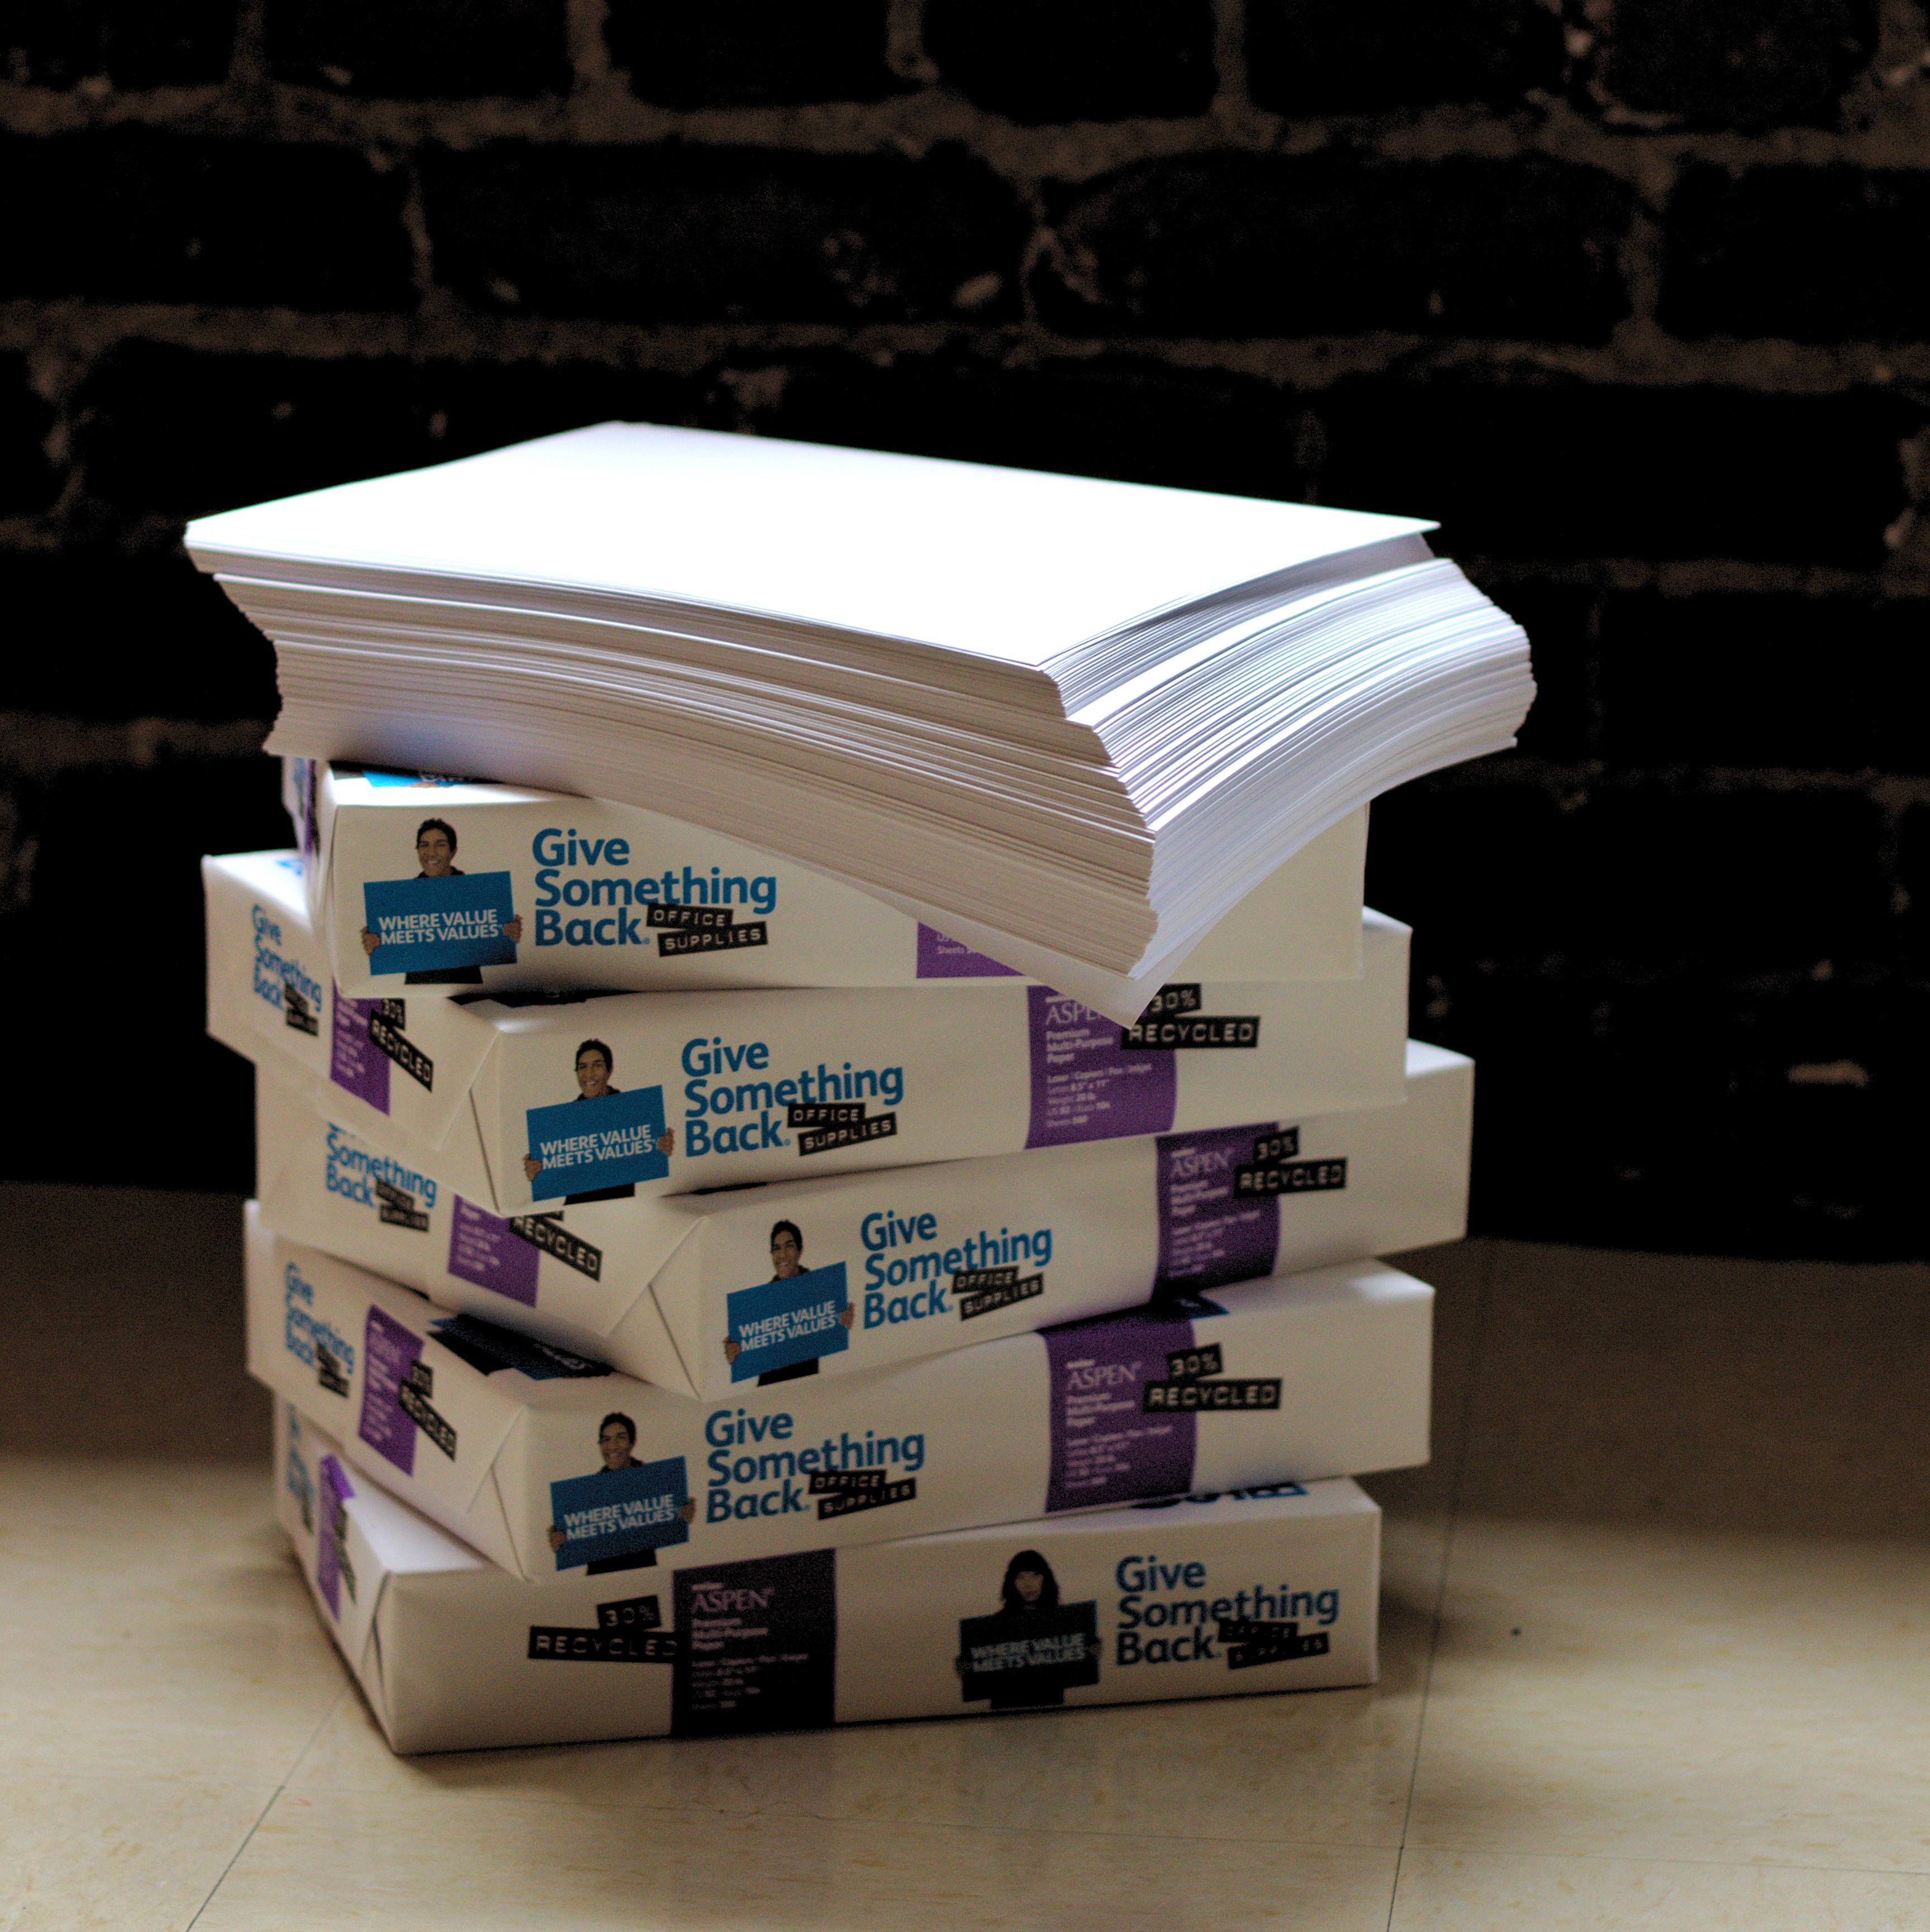
\includegraphics[width=0.75\columnwidth]{chapter15/figure14}\vspace{0.5cm}
\begin{center}\hspace{1cm}\chemfig{CH_3-CH_2-O-CH_2-CH_3}\end{center}
\caption{Diethyl ether was formerly used as a general anesthetic, until non-flammable drugs were developed. The image shows a panel from monument in Boston commemorating the demonstration of ether's anesthetic use.}
\end{marginfigure}%%%%%%% MARGIN FIGURE
\begin{marginfigure}[0cm]%%%%%%%% MARGIN FIGURE
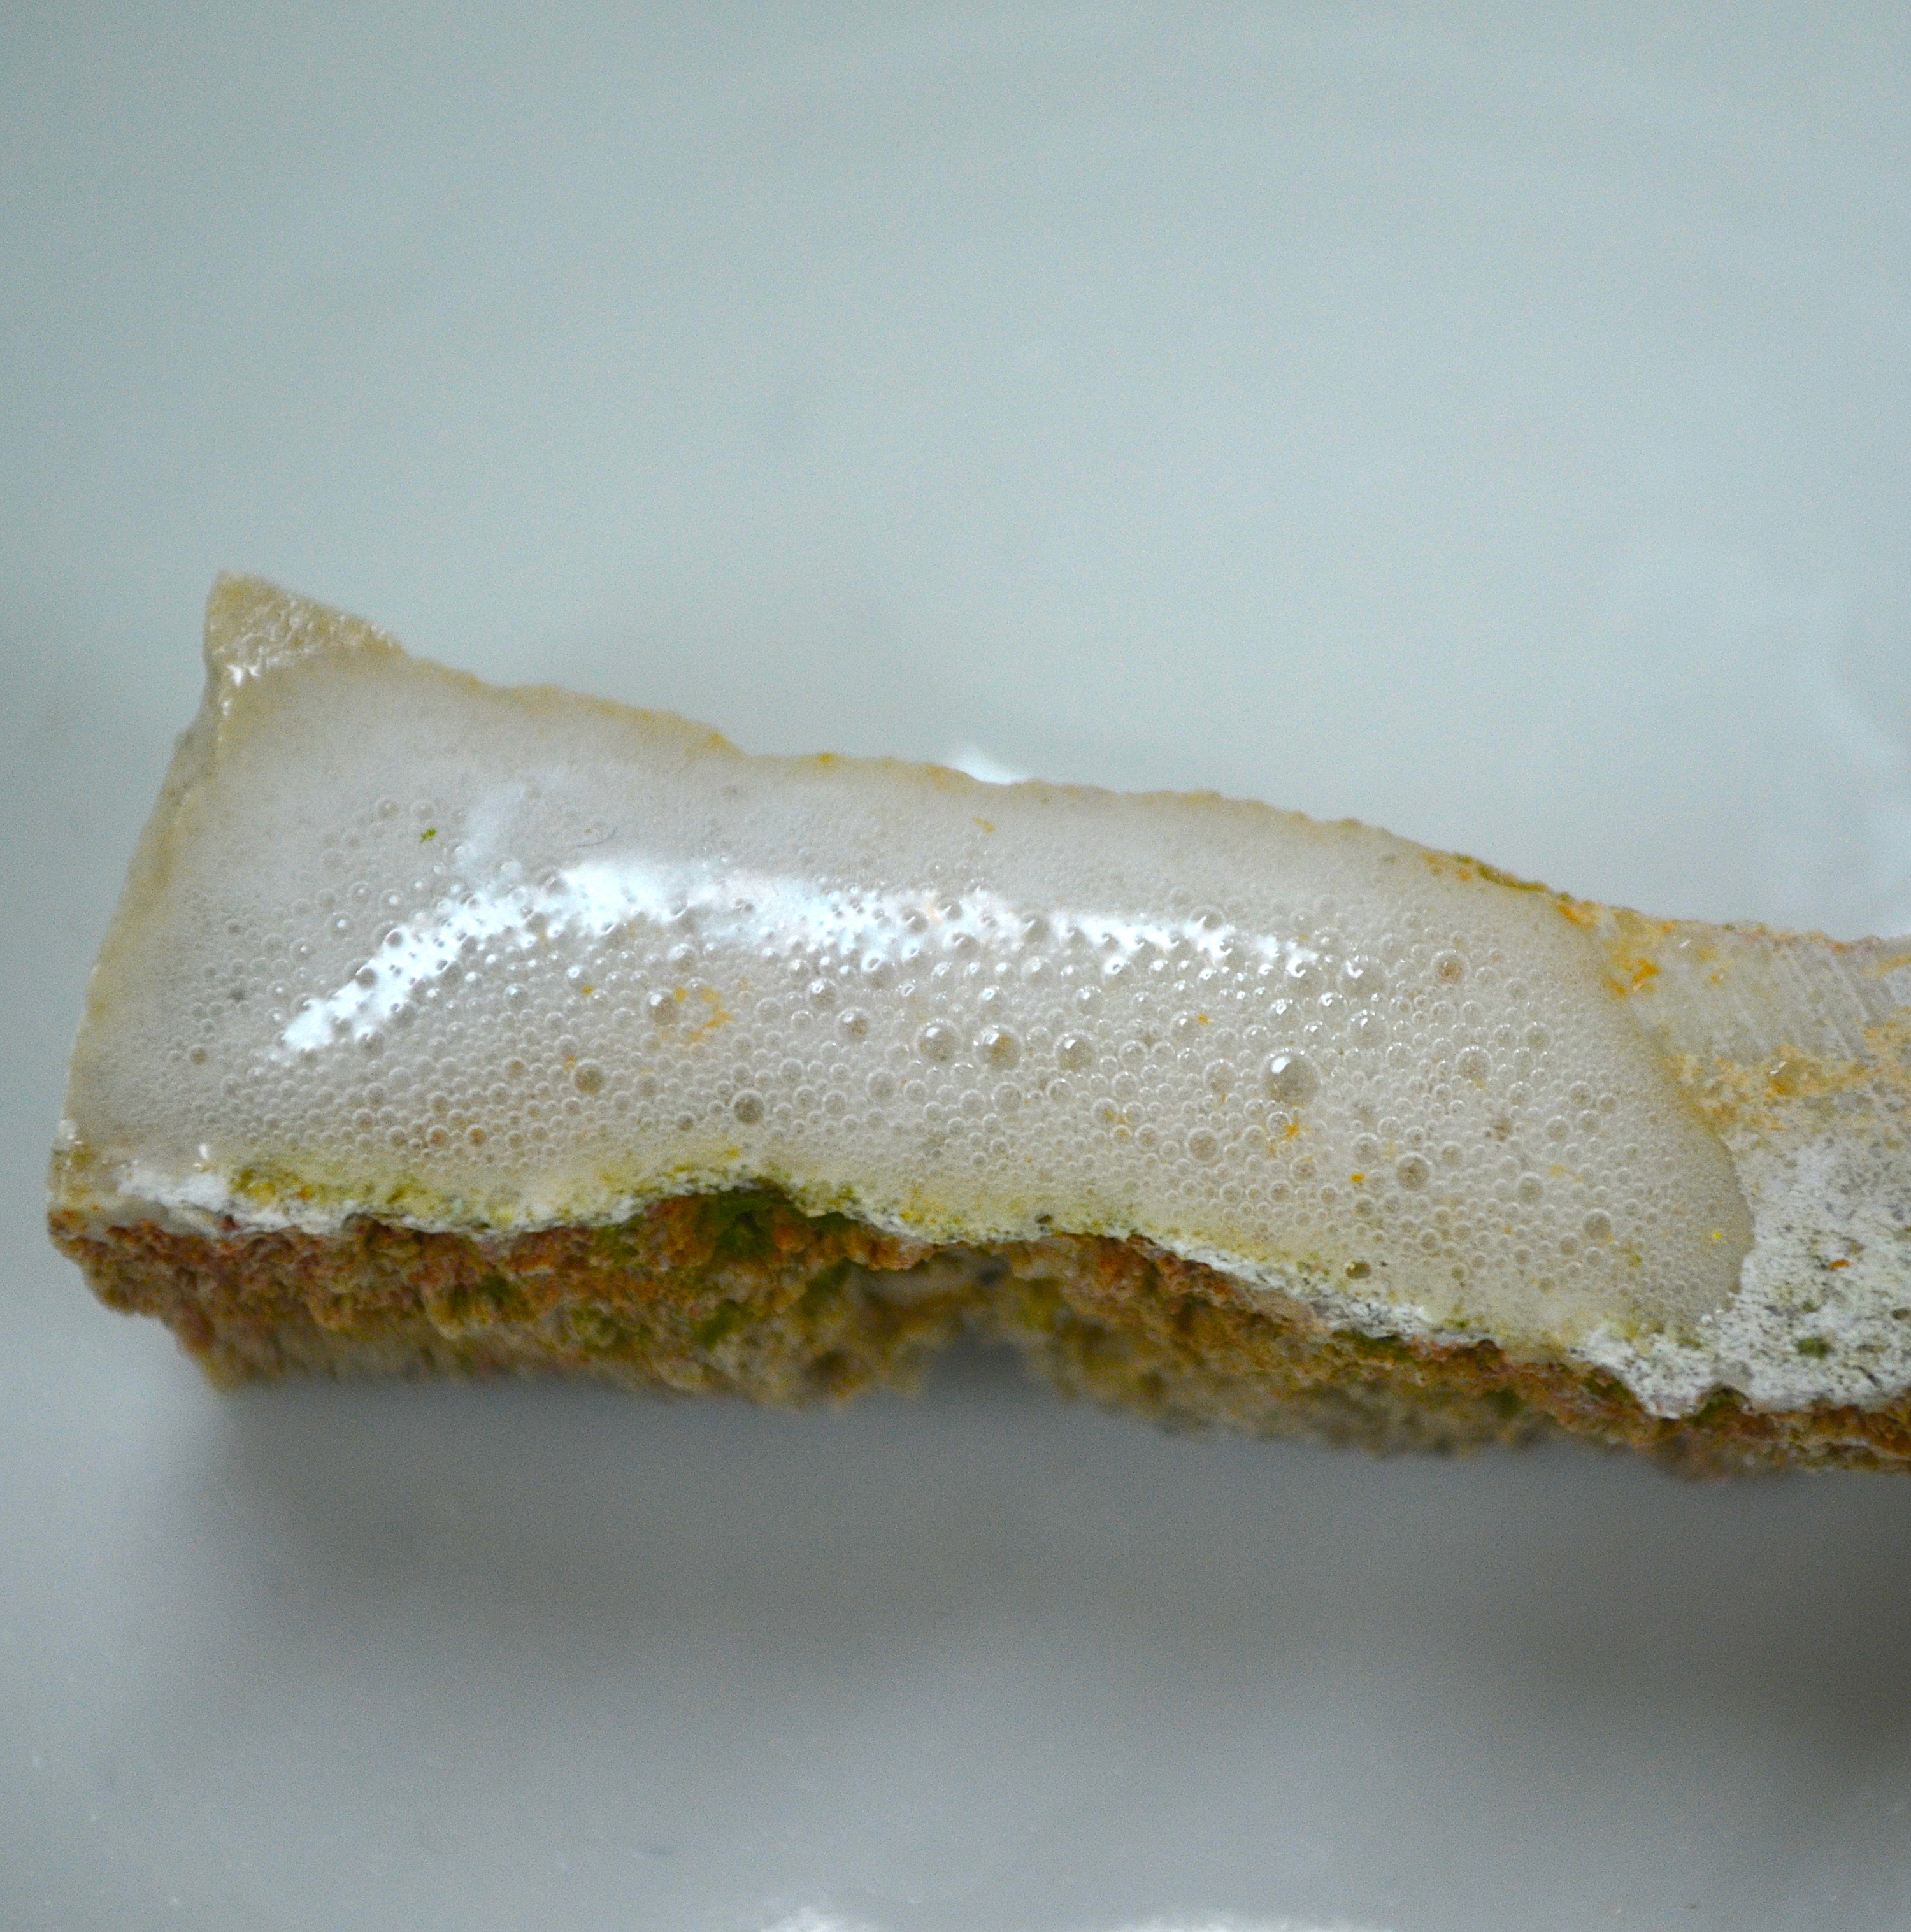
\includegraphics[width=1\columnwidth]{chapter15/figure11}\vspace{0.5cm}
\includegraphics[width=1\columnwidth]{chapter15/figure12}
\begin{center}\hspace{1cm}\chemfig{**6(---(-[:45]=[:-45]-[:45](=[:90]O)-[:-45]H)---)}\end{center}
\caption{Cinnamaldehyde is the aldehyde that gives cinnamon its flavor and odor.}
\end{marginfigure}%%%%%%% MARGIN FIGURE




\item[\docfilehook{\smallpencil Carboxylic acids and esters}{Carboxylic acids and esters}] Carboxylic acids contain a carbonyl group (\ce{C=O}) connected to an hydrocarbon and also an alcohol group:
\begin{center}\chemfig{R-C(=[:90]O)(-OH)}\hspace{0.5cm}\textcolor{blue}{Carboxylic acid}\end{center}
Esters have the same \ce{C=O} group but this time bounded to a carbon (R) and an ether group (\ce{-O-R^{'}}). 
\begin{center}\chemfig{R-C(=[:90]O)-O-R'}\hspace{0.5cm}\textcolor{blue}{Ester}\end{center}
Examples of carboxylic acids and esters are:
\begin{center}\chemname{\chemfig{CH_3-C(=[:90]O)(-OH)}}{Carboxylic acid}\hspace{1cm} or \hspace{1cm}\chemname{\chemfig{CH_3-C(=[:90]O)-O-CH_3}  }{Esters}\end{center}
\begin{example} %%%%%%%%%%%%%%%%%%%%%%%% EXAMPLE BOX
Classify the following molecules as an carboxylic acid or ester:
\begin{center}\chemfig{-[:45]-[:-45]-[:45](=[:90]O)(-[:-45]OH)} \hspace{0.5cm}\chemfig{-[:45]-[:-45](=[:-90]O)-[:45]O-[:-45]}  \end{center}
\textlcsc{ \textcolor{dgreen}{\Large \textbf{Solution}} }\\
The molecule in the left is a carboxylic acid as the carbonyl group (\ce{C=O}) is connected to an alcohol \ce{-OH}. Differently, the molecule in the right is a ester as the carbonyl group is connected to a \ce{-O-CH3} group.
\\
\faDiamond\ \textlcsc{ \textcolor{dgreen}{\Large \textbf{Study Check}} }\\
Classify the following molecules as an carboxylic acid or ester:
\begin{center}  \chemfig{*6(-(-[:-90]C(=[:-45]O)(-[:-135]O-CH_3))-----)}  \hspace{0.5cm}  \chemfig{*6(---(-C(=[:-45]O)(-[:45]OH))---)}   \end{center}

\flushright{  \small Answer: (left) ester; (right) acid. }
\end{example}%%%%%%%%%%%%%%%%%%%%%%%% EXAMPLE BOX


\begin{marginfigure}[0cm]%%%%%%%% MARGIN FIGURE
\includegraphics[width=0.75\columnwidth]{chapter15/figure15}\vspace{0.5cm}
\begin{center}\hspace{1cm}\chemfig{**6(---(-[:45]-[:-45]O-[:45](=[:90]O)-[:-45])---)}\end{center}
\caption{Benzyl acetate is an ester that flavors pears.}
\end{marginfigure}%%%%%%% MARGIN FIGURE
\begin{marginfigure}[0cm]%%%%%%%% MARGIN FIGURE
\includegraphics[width=0.75\columnwidth]{chapter15/figure16}\vspace{0.5cm}
\begin{center}\hspace{1cm}\chemfig{-[:45]-[:-45]-[:45](=[:90]O)-[:-45]O-[:45]-[:-45]-[:45]-[:-45]}\end{center}
\caption{Butyl butyrate is an ester that flavors pinapple.}
\end{marginfigure}%%%%%%% MARGIN FIGURE
%\begin{marginfigure}[0cm]%%%%%%%% MARGIN FIGURE
%\includegraphics[width=0.75\columnwidth]{chapter15/figure17}\vspace{0.5cm}
%\begin{center}\hspace{1cm}\chemfig{-[:45](-[:90])-[:-45]-[:45](=[:90]O)-[:-45]O-[:45]-[:-45]-[:45]-[:-45]}\end{center}
%\caption{Ethyl isovalerate is an ester that flavors apples.}
%\end{marginfigure}%%%%%%% MARGIN FIGURE

\item[\docfilehook{\smallpencil Amines and amides}{Amines and amides}] Amines and amides are groups containing nitrogen. Amines are derivative of ammonia (\ce{NH3}) with one or more of the hydrogen atoms being replaced by a hydrocarbon
\begin{center}\chemfig{R-N(-[:90]R')(-R'')}\hspace{0.5cm}\textcolor{blue}{Amine}\end{center}
 All these molecules are amines:
\begin{center}\chemfig{CH_3-N(-H)(-[:90]CH_3)}\hspace{1cm}  \chemfig{CH_3-NH_2} \hspace{1cm}  \chemfig{CH_3-N(-CH_2CH_3)(-[:90]CH_3)} \end{center}
Amides, on the other hand, contain a carbonyl group (\ce{C=O}) connected to an amine group (\chemfig{-N(-)(-[:90])})
\begin{center}  \chemfig{R-C(=[:90]O)(-N(-R')((-[:90]R'')))}  \hspace{0.5cm}\textcolor{blue}{Amide}\end{center}
Examples of amides are:
\begin{center}\chemfig{CH_3-C(=[:90]O)(-NH_2)}\hspace{1cm} or \hspace{1cm}\chemfig{CH_3-CH_2-C(=[:90]O)-N(-[:90]H)(-CH_3)}\end{center}

\begin{example} %%%%%%%%%%%%%%%%%%%%%%%% EXAMPLE BOX
Classify the following molecules as an amide or amine:
\begin{center}\chemfig{-[:45]-[:-45]-[:45](=[:90]O)(-[:-45]NH_2)} \hspace{0.5cm}\chemfig{-[:45]-[:-45]-[:45]N-[:-45]}  \end{center}
\textlcsc{ \textcolor{dgreen}{\Large \textbf{Solution}} }\\
The molecule in the left is a amide as the carbonyl group (\ce{C=O}) is connected to a nitrogen atom. Differently, the molecule in the right is an amine as the nitrogen group is not connected to any carbonyl group.
\\
\faDiamond\ \textlcsc{ \textcolor{dgreen}{\Large \textbf{Study Check}} }\\
Classify the following molecules as an amide or amine:
\begin{center}  \chemfig{*6(-(-[:-90]C(=[:-45]O)(-[:-135]N(-CH_3)(-[:180]CH_3)))-----)}  \hspace{0.5cm}  \chemfig{*6(---(-N(-[:-45]CH_3)(-CH_3))---)}   \end{center}

\flushright{  \small Answer: (left) amide; (right) amine. }
\end{example}%%%%%%%%%%%%%%%%%%%%%%%% EXAMPLE BOX







\end{description}









\end{document}
%    coordinates {(0,20) (8,5) (24,2.5) (32,1.25) (40,0.6)} ;
%    \node [above] at (axis cs:  8,5) {$t_{1/2}$};
%        \node [above] at (axis cs:  24,2.5) {$2t_{1/2}$};
%        \node [above] at (axis cs:  32,1.25) {$3t_{1/2}$};
%\end{axis}
%    \end{tikzpicture}
%\end{marginfigure}%%%%%%%MARGIN PLOT
